\documentclass[../main.tex]{subfiles}

\begin{document}
\part*{Initial-Value Problems}

\vspace{1,5in}

\begin{center}\begin{Large}\textbf{CHAPTER OBJECTIVES}\end{Large}\end{center}
The primary objective of this chapter is to introduce you to numerical differentiation.
Specific objectives and topics covered are

\begin{itemize}
	\item Understanding the meaning of local and global truncation errors and their
relationship to step size for one-step methods for solving ODEs.
	\item Knowing how to implement the following Runge-Kutta (RK) methods for 
a single ODE:\\
Euler\\
Heun\\
Midpoint\\
Fourth-order RK
	\item Knowing how to iterate the corrector of Heun's method.
	\item Knowing how to implement the following Runge-Kutta methods for systems of ODEs:\\
Euler\\
Fourth-order RK\\
\end{itemize}
\vspace{0.3in}
\begin{Large}\textbf{YOU'VE GOT A PROBLEM}\end{Large}\\
We started this book with the problem of simulating the velocity of a free-falling
bungee jumper. This problem amounted to formulating and solving an ordinary
differential equation, the topic of this chapter. Now let's return to this problem
and make it more interesting by computing what happens when the jumper reaches the end
of the bungee cord.

To do this, we should recognize that the jumper will experience different forces depending on whether the cord is slack or stretched. If it is slack, the situation is that of free
fall where the only forces are gravity and drag. However, because the jumper can now
move up as well as down, the sign of the drag force must be modified so that it always tends
to retard velocity,
\begin{equation}
\tag{22.1a}
\dfrac{dv}{dt} = g - sign(v)\dfrac{c_{d}}{m}v^2
\end{equation}\\
where v is velocity (m/s), $t$ is time (s), g is the acceleration due to gravity ($9.81 m/s^2$), cd is
the drag coefficient (kg/m), and $m$ is mass (kg). The signum function\footnotemark, sign, returns a −1 or
a 1 depending on whether its argument is negative or positive, respectively. Thus, when the
jumper is falling downward (positive velocity, sign = 1), the drag force will be negative
and hence will act to reduce velocity. In contrast, when the jumper is moving upward
(negative velocity, sign = −1), the drag force will be positive so that it again reduces the
velocity.

\footnotetext{Some computer languages represent the signum function as \texttt{sgn(x)}. As represented here, MATLAB uses the
nomenclature \texttt{sign(x)}}

Once the cord begins to stretch, it obviously exerts an upward force on the jumper. As
done previously in Chap. 8, Hooke's law can be used as a first approximation of this force.
In addition, a dampening force should also be included to account for frictional effects as
the cord stretches and contracts. These factors can be incorporated along with gravity and
drag into a second force balance that applies when the cord is stretched. The result is the
following differential equation:
\begin{equation}
\tag{22.1b}
\dfrac{dv}{dt} = g - sign(v) \dfrac{c_{d}}{m} v^2 - \dfrac{k}{m} (x-L) - \dfrac{\gamma}{m}v
\end{equation}\\
where $k$ is the cord's spring constant (N/m), $x$ is vertical distance measured downward from
the bungee jump platform (m), $L $is the length of the unstretched cord (m), and $\gamma$ is a dampening coefficient (N · s/m).

Because Eq. (22.1b) only holds when the cord is stretched ($x > L$), the spring force
will always be negative. That is, it will always act to pull the jumper back up. The dampening force increases in magnitude as the jumper's velocity increases and always acts to
slow the jumper down.

If we want to simulate the jumper's velocity, we would initially solve Eq. (22.1a) until
the cord was fully extended. Then, we could switch to Eq. (22.1b) for periods that the cord
is stretched. Although this is fairly straightforward, it means that knowledge of the
jumper's position is required. This can be done by formulating another differential equation for distance:\\
\begin{equation}
\tag{22.2}
\dfrac{dx}{dt} = v
\end{equation}

Thus, solving for the bungee jumper's velocity amounts to solving two ordinary differential equations where one of the equations takes different forms depending on the value of one of the dependent variables. Chapters 22 and 23 explore methods for solving this and
similar problems involving ODEs.

\vspace{0,6in}
\section{22.1 OVERVIEW}
\vspace{0,1in}
\hrule
\vspace{0,1in}
This chapter is devoted to solving ordinary differential equations of the form
\begin{equation}
\tag{22.3}
\dfrac{dy}{dt} = f(t,y)
\end{equation}\\
where the slope $\phi$ is called an $increment function$. According to this equation, the slope estimate of $\phi$ is used to extrapolate from an old value $y_{i}$ to a new value $y_{i+1}$ over a distance $h$ This formula can be applied step by step to trace out the trajectory of the solution into
the future. Such approaches are called $one-step methods$ because the value of the increment
function is based on information at a single point $i$. They are also referred to as $RungeKutta methods$ after the two applied mathematicians who first discussed them in the early
1900s. Another class of methods called $multistep methods$ use information from several
previous points as the basis for extrapolating to a new value. We will describe multistep
methods briefly in Chap. 23.

All one-step methods can be expressed in the general form of Eq. (22.4), with the only
difference being the manner in which the slope is estimated. The simplest approach is to
use the differential equation to estimate the slope in the form of the first derivative at ti . In
other words, the slope at the beginning of the interval is taken as an approximation of the
average slope over the whole interval. This approach, called Euler's method, is discussed
next. This is followed by other one-step methods that employ alternative slope estimates
that result in more accurate predictions.

\vspace{0,6in}
\section{22.2 EULER'S METHOD}
\vspace{0,1in}
\hrule
\vspace{0,1in}
The first derivative provides a direct estimate of the slope at $t_{i}$ (Fig. 22.1):
\begin{equation}
\tag{22.5}
y_{i+1} = y_{i} + f(t_{i},y_{i})h
\end{equation}\\
This formula is referred to as $Euler's method$ (or the Euler-Cauchy or point-slope method).
A new value of $y$ is predicted using the slope (equal to the first derivative at the original
value of $t$) to extrapolate linearly over the step size h (Fig. 22.1).\\
\begin{figure}[hbt!]
	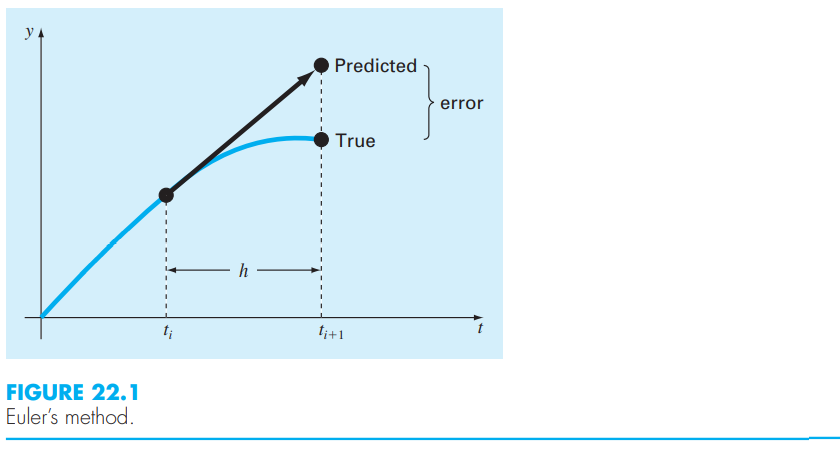
\includegraphics[width=0.95\textwidth]{F22_1}
	\label{F 22.1}
\end{figure}\\

\vspace{0,3in}
\section{Euler's Method}
\vspace{0,1in}
\hrule
\vspace{0,1in}
\textbf{Problem Statement.} Use Euler's method to integrate $y' = 4e^{0.8t} - 0.5y$ from $t = 0$ to 4 with a step size of 1. The initial condition at $t$ = 0 is $y$ = 2. Note that the exact solution can
be determined analytically as\\

$y= \dfrac{4}{1.3} (e^{0.8t} - e^{-0.5t}) + 2e^{-0.5t} $

\vspace{0.2in}
\textbf{Solution.} Equation (22.5) can be used to implement Euler's method:

$y(1) = y(0) + f(0,2)(1)$\\

where $y(0) = 2$ and the slope estimate at $t$ = 0 is\\

$f(0,2) = 4e^0 - 0.5(2) = 3$\\

Therefore,\\

$y(1) = 2 + 3(1) = 5$\\

The true solution at $t$ = 1 is\\

$y=\dfrac{4}{1.3} \left(e^{0.8(1)} - e^{-0.5(1)} \right) + 2e^{-0.5(1)} = 6.19463$\\

Thus, the percent relative error is\\

$\varepsilon_{t} = \left| \dfrac{6.19463 - 5}{6.19463} \right| x 100 \% = 19.28 \% $\\

For the second step:\\

$y(2) = y(1) + f(1,5)(1)$
$$= 5 + [4e^{0.8(1)} - 0.5(5)](1) = 11.40216 $$


\vspace{0,3in}
\textbf{Table 22.1}
Comparison of true and numerical values of the integral
of $y' = 4e^{0.8t} - 0.5y$, with the initial condition that $y = 2$ at $t = 0$. The numerical values were computed using Euler's
method with a step size of 1.\\
\begin{tabular}{lccc}
\hline

	\textbf{$t$} \; \; \; \; \; & \textbf{$y_{true}$} \; \; \; \; \; & \textbf{$y_{Euler}$} \; \; \; \; \; &  \textbf{$\left|\varepsilon_{t}\right|( \% )$}\\
	
\hline

	0 \; \; \; \; \; & 2.00000 \; \; \; \; \; & 2.00000 \; \; \; \; \; & \vspace{0in}\\
	
	1 \; \; \; \; \; & 6.19463 \; \; \; \; \; & 5.00000 \; \; \; \; \; & 19.28\\

	2 \; \; \; \; \; & 14.84392 \; \; \; \; \; & 11.40216 \; \; \; \; \; & 23.19\\

	3 \; \; \; \; \; & 33.67717 \; \; \; \; \; & 25.51321 \; \; \; \; \; & 24.24\\

	4 \; \; \; \; \; & 75.33896 \; \; \; \; \; & 56.84931 \; \; \; \; \; & 24.54\\

\hline
\end{tabular}


\begin{figure}[hbt!]
	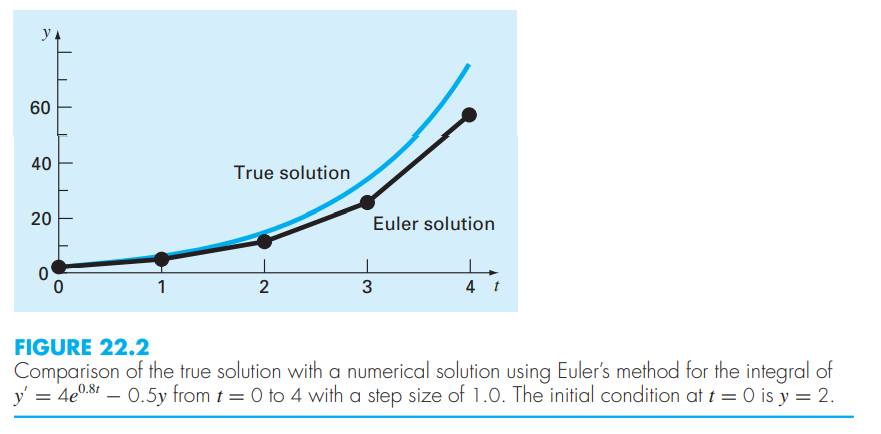
\includegraphics[width=0.95\textwidth]{F22_2}
	\label{F22.2}
\end{figure}
The true solution at t = 2.0 is 14.84392 and, therefore, the true percent relative error is
23.19\%. The computation is repeated, and the results compiled in Table 22.1 and Fig. 22.2.
Note that although the computation captures the general trend of the true solution, the error
is considerable. As discussed in the next section, this error can be reduced by using a
smaller step size.

\subsection{Error Analysis for Euler's Method}

The numerical solution of ODEs involves two types of error (recall Chap. 4):
\begin{enumerate}
\item $Truncation$, or discretization, errors caused by the nature of the techniques employed
to approximate values of $y$.
\item $Roundoff$ errors caused by the limited numbers of significant digits that can be retained
by a computer.
\end{enumerate}

The truncation errors are composed of two parts. The first is a local truncation error that results from an application of the method in question over a single step. The second is
a propagated truncation error that results from the approximations produced during the previous steps. The sum of the two is the total error. It is referred to as the global truncation error.

Insight into the magnitude and properties of the truncation error can be gained by deriving Euler's method directly from the Taylor series expansion. To do this, realize that the
differential equation being integrated will be of the general form of Eq. (22.3), where
$dy/dt = y$, and $t$ and $y$ are the independent and the dependent variables, respectively. If
the solution—that is, the function describing the behavior of $y$—has continuous derivatives,
it can be represented by a Taylor series expansion about a starting value ($t_{i}$, $y_{i}$), as in
[recall Eq. (4.13)]:\\
\begin{equation}
\tag{22.6}
y_{i+1} = y_{i} + y^{'}_{i}h + \dfrac{y^{"}_{i}}{2!}h^2 + \cdots + \dfrac{y^{(n)}_{i}}{n!}h^n + R_{n}
\end{equation}\\
where $h = t_{i+1} − t_{i}$ and $R_{n}$ = the remainder term, defined as\\
\begin{equation}
\tag{22.7}
R_{n} = \dfrac{y^{(n+1)}(\xi)}{(n+1)!}h^{n+1}
\end{equation}\\
where $\xi$ lies somewhere in the interval from $t_{i}$ to $t_{i+1}$. An alternative form can be developed by substituting Eq. (22.3) into Eqs. (22.6) and (22.7) to yield\\
\begin{equation}
\tag{22.8}
y_{i+1} = y_{i} + f(t_{i},y_{i})h + \dfrac{f^{'} (t_{i}, y_{i})}{2!}h^2 + \cdots + \dfrac{f^{(n-1)} (t_{i}, y_{i})}{n!}h^n + O(h^{n+1})
\end{equation}\\
where $O(h^{n+1})$ specifies that the local truncation error is proportional to the step size
raised to the ($n + 1$)th power.

By comparing Eqs. (22.5) and (22.8), it can be seen that Euler's method corresponds to the Taylor series up to and including the term $f(t_{i}, y_{i})h$. Additionally, the comparison
indicates that a truncation error occurs because we approximate the true solution using a finite number of terms from the Taylor series. We thus truncate, or leave out, a part of the true
solution. For example, the truncation error in Euler's method is attributable to the remaining terms in the Taylor series expansion that were not included in Eq. (22.5). Subtracting
Eq. (22.5) from Eq. (22.8) yields\\
\begin{equation}
\tag{22.9}
E_{t} = \dfrac{ f^{'}( t_{i},y_{i} ) }{2!}h^2 + \cdots + O(h^{n+1})
\end{equation}\\
where $E_{t}$ = the true local truncation error. For sufficiently small $h$, the higher-order terms
in Eq. (22.9) are usually negligible, and the result is often represented as\\
\begin{equation}
\tag{22.10}
E_{a} = \dfrac{f^{'} ( t_{i}, y_{i} )}{2!} h^2
\end{equation}\\
or\\
\begin{equation}
\tag{22.11}
E_{a} = O(h^2)
\end{equation}\\
where $E_{a}$ = the approximate local truncation error.

According to Eq. (22.11), we see that the local error is proportional to the square of
the step size and the first derivative of the differential equation. It can also be demonstrated that the global truncation error is $O(h)$—that is, it is proportional to the step size (Carnahan et al., 1969). These observations lead to some useful conclusions:

\begin{enumerate}
\item The global error can be reduced by decreasing the step size.
\item The method will provide error-free predictions if the underlying function (i.e., the
solution of the differential equation) is linear, because for a straight line the second
derivative would be zero.
\end{enumerate}
This latter conclusion makes intuitive sense because Euler's method uses straight-line segments to approximate the solution. Hence, Euler's method is referred to as a first-order
method.


It should also be noted that this general pattern holds for the higher-order one-step
methods described in the following pages. That is, an nth-order method will yield perfect
results if the underlying solution is an nth-order polynomial. Further, the local truncation
error will be $O(h^{n+1})$ and the global error $O(h^n)$.

\subsection{Stability of Euler's Method}
In the preceding section, we learned that the truncation error of Euler's method depends on
the step size in a predictable way based on the Taylor series. This is an accuracy issue.

The stability of a solution method is another important consideration that must be considered when solving ODEs. A numerical solution is said to be unstable if errors grow
exponentially for a problem for which there is a bounded solution. The stability of a particular application can depend on three factors: the differential equation, the numerical
method, and the step size.

Insight into the step size required for stability can be examined by studying a very
simple ODE:\\
\begin{equation}
\tag{22.12}
\dfrac{dy}{dt} = -ay
\end{equation}\\
If $y(0) = y_{0}$, calculus can be used to determine the solution as\\

$y=y_{0}e^{-at}$\\
\\
Thus, the solution starts at $y_{0}$ and asymptotically approaches zero.

Now suppose that we use Euler's method to solve the same problem numerically:\\

$y_{i+1} = y_{i} + \dfrac{dy_{i}}{dt} h$
\\
Substituting Eq. (22.12) gives\\

$$y_{i+1} = y_{i} - ay_{i}h$$\\
or\\
\begin{equation}
\tag{22.13}
y_{i+1} = y_{i}(1-ah)
\end{equation}
The parenthetical quantity $1 − ah$ is called an $amplification factor$. If its absolute value is
greater than unity, the solution will grow in an unbounded fashion. So clearly, the stability
depends on the step size $h$. That is, if $ h > 2/a, |y_{i}| \rightarrow \infty$ as $ i \rightarrow \infty $. Based on this analysis, Euler's method is said to be $conditionally stable$.

Note that there are certain ODEs where errors always grow regardless of the method.
Such ODEs are called $ill-conditioned$.

Inaccuracy and instability are often confused. This is probably because (a) both represent situations where the numerical solution breaks down and (b) both are affected by step
size. However, they are distinct problems. For example, an inaccurate method can be very
stable. We will return to the topic when we discuss stiff systems in Chap. 23.

\subsection{MATLAB M-file Function: \texttt{eulode}}
We have already developed a simple M-file to implement Euler's method for the falling
bungee jumper problem in Chap. 3. Recall from Section 3.6, that this function used Euler's
method to compute the velocity after a given time of free fall. Now, let's develop a more
general, all-purpose algorithm.

Figure 22.3 shows an M-file that uses Euler's method to compute values of the dependent
variable \texttt{y} over a range of values of the independent variable \texttt{t}. The name of the function
holding the right-hand side of the differential equation is passed into the function as the\\
\begin{figure}[hbt!]
	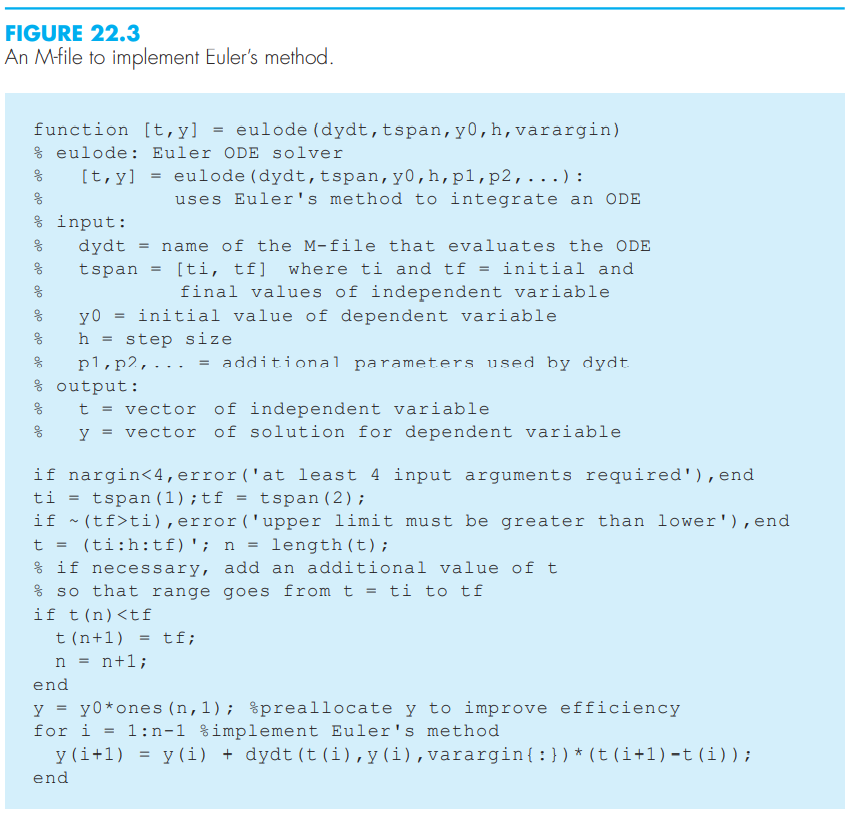
\includegraphics[width=0.85\textwidth]{F22_3}
	\label{F22.3}
\end{figure}\\
variable \texttt{dydt}. The initial and final values of the desired range of the independent variable
is passed as a vector \texttt{tspan}. The initial value and the desired step size are passed as \texttt{y0} and
h, respectively.

The function first generates a vector \texttt{t} over the desired range of the dependent variable
using an increment of \texttt{h}. In the event that the step size is not evenly divisible into the range,
the last value will fall short of the final value of the range. If this occurs, the final value is
added to \texttt{t} so that the series spans the complete range. The length of the \texttt{t} vector is determined as \texttt{n}. In addition, a vector of the dependent variable \texttt{y} is preallocated with \texttt{n} values
of the initial condition to improve efficiency.

At this point, Euler's method (Eq. 22.5) is implemented by a simple loop:

\begin{verbatim}
   for i = 1:n-1 
      y(i+1) = y(i) + dydt(t(i),y(i),varargin{:})*(t(i+1)-
   t(i));
   end
\end{verbatim}
Notice how a function is used to generate a value for the derivative at the appropriate values of the independent and dependent variables. Also notice how the time step is automatically calculated based on the difference between adjacent values in the vector \texttt{t}.

The ODE being solved can be set up in several ways. First, the differential equation can
be defined as an anonymous function object. For example, for the ODE from Example 22.1:

\begin{verbatim}
   >> dydt=@(t,y) 4*exp(0.8*t) - 0.5*y;
\end{verbatim}
The solution can then be generated as

\begin{verbatim}
   >> [t,y] = eulode(dydt,[0 4],2,1);
   >> disp([t,y])
\end{verbatim}
with the result (compare with Table 22.1):

\begin{verbatim}
        0  2.0000
   1.0000  5.0000
   2.0000  11.4022
   3.0000  25.5132
   4.0000  56.8493
\end{verbatim}

Although using an anonymous function is feasible for the present case, there will be
more complex problems where the definition of the ODE requires several lines of code. In
such instances, creating a separate M-file is the only option.

\vspace{0,3in}
\section{22.3 IMPROVEMENTS OF EULER'S METHOD}
\vspace{0,1in}
\hrule
\vspace{0,1in}

A fundamental source of error in Euler's method is that the derivative at the beginning of
the interval is assumed to apply across the entire interval. Two simple modifications are
available to help circumvent this shortcoming. As will be demonstrated in Section 22.4,
both modifications (as well as Euler's method itself) actually belong to a larger class of solution techniques called Runge-Kutta methods. However, because they have very straightforward graphical interpretations, we will present them prior to their formal derivation as
Runge-Kutta methods.

\subsection{Heun's Method}
One method to improve the estimate of the slope involves the determination of two derivatives for the interval—one at the beginning and another at the end. The two derivatives are
then averaged to obtain an improved estimate of the slope for the entire interval. This approach, called $Heun's method$, is depicted graphically in Fig. 22.4.

Recall that in Euler's method, the slope at the beginning of an interval

\begin{equation}
\tag{22.14}
y^{'}_{i} = f(t_{i},y_{i})
\end{equation}\\
is used to extrapolate linearly to $y_{i+1}$:

\begin{equation}
\tag{22.15}
y^{0}_{i+1} = y_{i} + f( t_{i}, y_{i} )h
\end{equation}\\
For the standard Euler method we would stop at this point. However, in Heun's method the $y^{0}_{i+1}$ calculated in Eq. (22.15) is not the final answer, but an intermediate prediction. This is
why we have distinguished it with a superscript 0. Equation (22.15) is called a $predictor equation$. It provides an estimate that allows the calculation of a slope at the end of the interval:

\begin{equation}
\tag{22.16}
y^{'}_{i+1} = f( t_{i+1},y^{0}_{i+1})
\end{equation}\\
Thus, the two slopes [Eqs. (22.14) and (22.16)] can be combined to obtain an average slope
for the interval:


$$\overline{y}^{'} = \dfrac{f(t_{i},y_{i} ) + f(t_{i+1}, y^{0}_{i+1}) }{2}$$


This average slope is then used to extrapolate linearly from $y_{i}$ to $y_{i+1}$ using Euler's
method:

\begin{equation}
\tag{22.17}
y_{i+1} = y_{i} + \dfrac{f(t_{i},y_{i} ) + f(t_{i+1}, y^{0}_{i+1}) }{2}h
\end{equation}\\
which is called a corrector equation.\\
\begin{figure}[hbt!]
	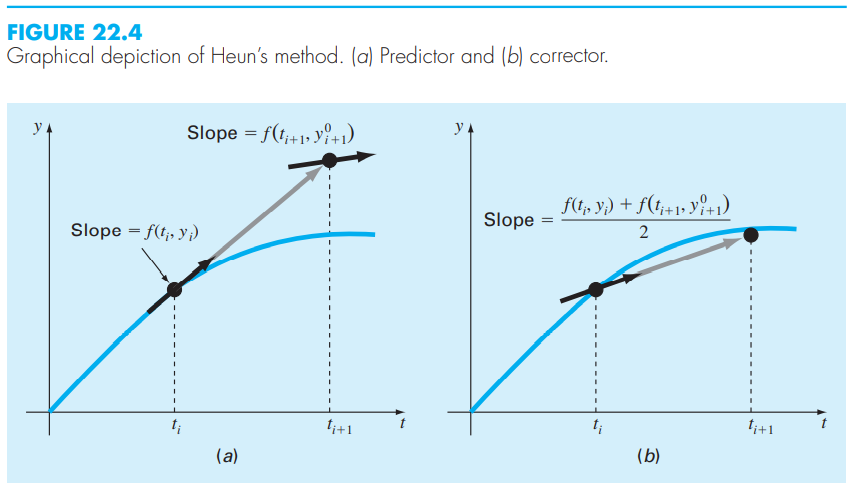
\includegraphics[width=0.85\textwidth]{F22_4}
	\label{F22.4}
\end{figure}\\

\begin{figure}[hbt!]
	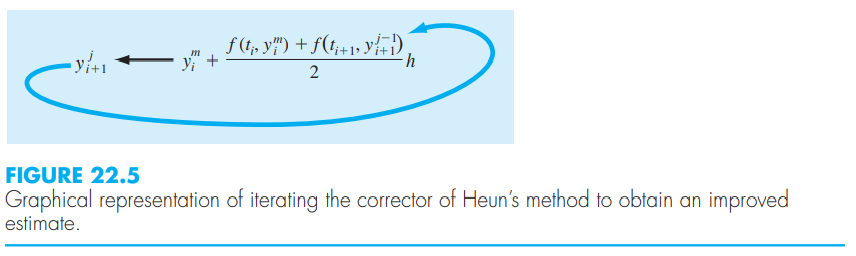
\includegraphics[width=0.85\textwidth]{F22_5}
	\label{F22.5}
\end{figure}

The Heun method is a $predictor-corrector$ approach. As just derived, it can be expressed concisely as

\begin{equation}
\tag{22.18}
\textnormal{Predictor (Fig. 22.4a):} \; \; \; \; \; \; \; y^{0}_{i+1} = y^{m}_{i} + f(t_{i}, y_{i})h
\end{equation}
\begin{equation}
\tag{22.19}
\textnormal{Corrector (Fig. 22.4b):} \; \; \; \; \; \; \; y^{j}_{i+1} = y^{m}_{i} + \dfrac{ f(t_{i},y^{m}_{i}) + f(t_{i+1},y^{j-1}_{i+1}) }{ 2 }h
\textnormal{(for j = 1, 2, . . . , m)}
\end{equation}
Note that because Eq. (22.19) has $y_{i+1}$ on both sides of the equal sign, it can be applied in
an iterative fashion as indicated. That is, an old estimate can be used repeatedly to provide
an improved estimate of $y_{i+1}$ The process is depicted in Fig. 22.5.

As with similar iterative methods discussed in previous sections of the book, a termination criterion for convergence of the corrector is provided by
\\

$|\xi_{a}| = \left| \dfrac{y^{j}_{i+1} - y^{j-1}_{i+1}}{y^{j}_i+1} \right| x 100\% $
\\
\\
where $y^{j-1}_{i+1}$ and $y^{j}_{i+1}$ are the result from the prior and the present iteration of the corrector,
respectively. It should be understood that the iterative process does not necessarily converge on the true answer but will converge on an estimate with a finite truncation error, as
demonstrated in the following example.\\

\vspace{0,3in}
\section{Heun's Method}
\vspace{0,1in}
\hrule
\vspace{0,1in}
\textbf{Problem Statement.} Use Heun's method with iteration to integrate $y^{'} = 4e^{0.8t} - 0.5y$ from t = 0 to 4 with a step size of 1. The initial condition at t = 0 is y = 2. Employ a stopping criterion of 0.00001\% to terminate the corrector iterations.
\\
\vspace{0.2in}\\
\textbf{Solution.} First, the slope at ($t_{0}, y_{0}$) is calculated as\\

$y^{'}_{0} = 4e^0 - 0.5(2) = 3$\\
\\
Then, the predictor is used to compute a value at 1.0:\\

$y^{0}_{1} = 2 + 3(1) = 5$\\

\vspace{0,3in}
\textbf{Table 22.1} Comparison of true and numerical values of the integral of $y^{'} = 4e^{0.8t} - 0.5y$, with the initial condition that $y=2$ at $t=0$. The numerical values
were computed using the Euler and Heun methods with a step size of 1.
The Heun method was implemented both without and with iteration of
the corrector.\\
\hrule
\begin{flushright}
\underline{Without Iteration} \; \; \underline{With Iteration}
\end{flushright} 
\begin{tabular}{lccccccc}
\textbf{$t$} \; \; \; \; & \textbf{$y_{true}$} \; \; \; \; & \textbf{$y_{Euler}$} \; \; \; \; & \textbf{$|\xi_{t}|(\%)$} \; \; \; \; &  \textbf{$y_{Heun}$} \; \; \; \; & \textbf{$|\xi_{t}|(\%)$} \; \; \; \; & \textbf{$y_{Heun}$} \; \; \; \; & \textbf{$|\xi_{t}|(\%)$}\\
\hline
0 & 2.00000 & 2.00000 & \vspace{0in} & 2.00000 & \vspace{0in} & 2.00000 & \vspace{0in}\\

1 & 6.19463 & 5.00000 & 19.28 & 6.70108 & 8.18 & 6.36087 & 2.68\\

2 & 14.84392 & 11.40216 & 23.19 & 16.31978 & 9.94 & 15.30224 & 3.09\\

3 & 33.67717 & 25.51321 & 24.24 & 37.19925 & 10.46 & 34.74328 & 3.17\\

4 & 75.33896 & 56.84931 & 24.54 & 83.33777 & 10.62 & 77.73510 & 3.18\\
\hline
\end{tabular}
\vspace{0,1in}
\\
Note that this is the result that would be obtained by the standard Euler method. The true
value in Table 22.2 shows that it corresponds to a percent relative error of 19.28\%.

Now, to improve the estimate for $y_{i+1}$, we use the value $y^0_1$ to predict the slope at the
end of the interval\\

$y^{'}_{1} = f(x_{1}, y^0_1) = 4e^{0.8(1)} - 0.5(5) = 6.402164$
\\
\\
which can be combined with the initial slope to yield an average slope over the interval
from t = 0 to 1:\\


$\overline{y}^{'} = \dfrac{3 + 6.402164}{2} = 4.701082$
\\
\\
This result can then be substituted into the corrector [Eq. (22.19)] to give the prediction at
t = 1:\\

$y^1_1 = 2 + 4.701082(1) = 6.701082$\\
\\
which represents a true percent relative error of −8.18\%. Thus, the Heun method without
iteration of the corrector reduces the absolute value of the error by a factor of about 2.4 as
compared with Euler's method. At this point, we can also compute an approximate error as\\

$ |\xi_{a}| = \left| \dfrac{6.701082 − 5}{6.701082} \right| x 100\% = 25.39\% $\\


Now the estimate of y1 can be refined by substituting the new result back into the
right-hand side of Eq. (22.19) to give\\

$^2_1 = 2 + \dfrac{3 + 4e^{0.8(1)} - 0.5(6.701082)}{2} 1 = 6.275811$\\
\\
which represents a true percent relative error of 1.31 percent and an approximate error of\\

$|\xi_{a}| = \left| \dfrac{6.275811 − 6.701082}{6.275811} \right| x 100\% = 6.776\%$\\
\\
The next iteration gives\\
\\
$y^2_1 = 2 + \dfrac{3 + 4e^{0.8(1)} - 0.5(6.275811)}{2}1 = 6.382129$\\
\\
which represents a true error of 3.03\% and an approximate error of 1.666\%.

The approximate error will keep dropping as the iterative process converges on a stable final result. In this example, after 12 iterations the approximate error falls below the
stopping criterion. At this point, the result at t = 1 is 6.36087, which represents a true relative error of 2.68\%. Table 22.2 shows results for the remainder of the computation along
with results for Euler's method and for the Heun method without iteration of the corrector.
\hrule

Insight into the local error of the Heun method can be gained by recognizing that it is
related to the trapezoidal rule. In the previous example, the derivative is a function of both
the dependent variable y and the independent variable t. For cases such as polynomials,
where the ODE is solely a function of the independent variable, the predictor step
[Eq. (22.18)] is not required and the corrector is applied only once for each iteration. For
such cases, the technique is expressed concisely as

\begin{equation}
\tag{22.20}
y_{i+1} = y_{i} + \dfrac{f(t_{i}) + f(t_{i+1})}{2}h
\end{equation}\\
\\
Notice the similarity between the second term on the right-hand side of Eq. (22.20) and the
trapezoidal rule [Eq. (19.11)]. The connection between the two methods can be formally
demonstrated by starting with the ordinary differential equation

\begin{equation}
\tag{22.21}
\dfrac{dy}{dt} = f(t)
\end{equation}\\
\\
This equation can be solved for y by integration:

\begin{equation}
\tag{22.22}
\int^{y_{i+1}}_{y_{i}} dy = \int^{t_{i+1}}_{t_{i}} f(t)dt
\end{equation}\\
\\
which yields

\begin{equation}
\tag{22.23}
y_{i+1} - y_{i} = \int^{t_{i+1}}_{t_{i}} f(t)dt
\end{equation}\\
\\
or

\begin{equation}
\tag{22.24}
y_{i+1} = y_{1} + \int^{t_{i+1}}_{t_{i}} f(t)dt
\end{equation}\\
\\
Now, recall that the trapezoidal rule [Eq. (19.11)] is defined as


\begin{equation}
\tag{22.25}
\int^{t_{i+1}}_{t_{i}} f(t)dt = \dfrac{f(t_{i})+ f(t_{i+1})}{2}h
\end{equation}\\
\\
where $h = t_{i+1} - t_{i}$. Substituting Eq. (22.25) into Eq. (22.24) yields

\begin{equation}
\tag{22.26}
y_{i+1} = y_{i} + \dfrac{f(t_{i}) + f(t_{i+1}) }{2}h
\end{equation}\\
\\
which is equivalent to Eq. (22.20). For this reason, Heun's method is sometimes referred to
as the trapezoidal rule.

Because Eq. (22.26) is a direct expression of the trapezoidal rule, the local truncation
error is given by [recall Eq. (19.14)]

\begin{equation}
\tag{22.27}
E_{t} = - \dfrac{f^{"}(\xi)}{12} h^3
\end{equation}\\
\\
where $\xi$ is between $t_{i}$ and $t_{i+1}$. Thus, the method is second order because the second derivative of the ODE is zero when the true solution is a quadratic. In addition, the local and
global errors are $O(h^3)$ and $O(h^2)$, respectively. Therefore, decreasing the step size
decreases the error at a faster rate than for Euler's method.

\subsection{The Midpoint Method}

Figure 22.6 illustrates another simple modification of Euler's method. Called the $midpoint method$, this technique uses Euler's method to predict a value of y at the midpoint of the
interval (Fig. 22.6a):

\begin{equation}
\tag{22.28}
y_{i+1/2} = y_{i} + f(t_{i},y_{i})\dfrac{h}{2}
\end{equation}\\
\\
Then, this predicted value is used to calculate a slope at the midpoint:

\begin{equation}
\tag{22.29}
y^{'}_{i+1/2} = f( t_{i+1/2}, y_{i+1/2} )
\end{equation}\\
\\
\begin{figure}[hbt!]
	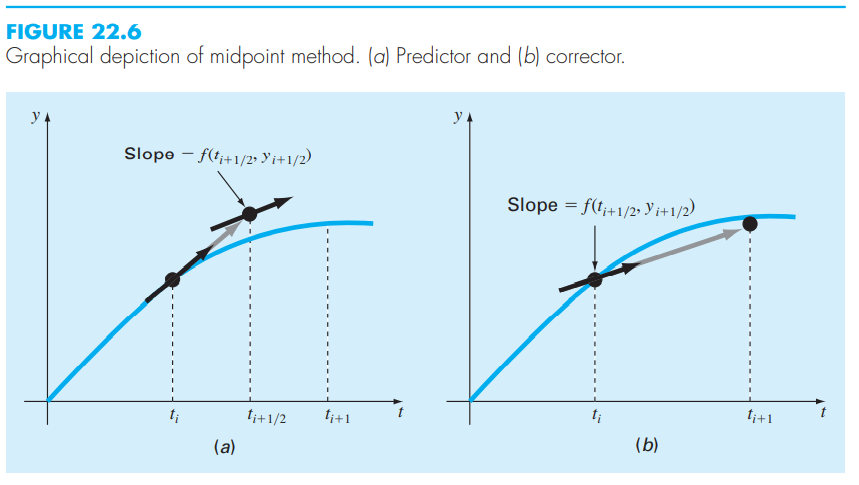
\includegraphics[width=0.85\textwidth]{F22_6}
	\label{F22.6}
\end{figure}\\
\\
which is assumed to represent a valid approximation of the average slope for the entire
interval. This slope is then used to extrapolate linearly from $t_{i}$ to $t_{i+1}$ (Fig. 22.6b):

\begin{equation}
\tag{22.30}
y_{i+1} = y_{1} + f( t_{i+1/2}, y_{i+1/2})h
\end{equation}\\
\\
Observe that because $_{i+1}$ is not on both sides, the corrector [Eq. (22.30)] cannot be applied
iteratively to improve the solution as was done with Heun's method.

As in our discussion of Heun's method, the midpoint method can also be linked to
Newton-Cotes integration formulas. Recall from Table 19.4 that the simplest Newton-Cotes
open integration formula, which is called the midpoint method, can be represented as

\begin{equation}
\tag{22.31}
\int^b_a f(x)dx \cong (b-a)f(x_{1})
\end{equation}\\
\\
where $x_{1}$ is the midpoint of the interval ($a, b$). Using the nomenclature for the present case,
it can be expressed as

\begin{equation}
\tag{22.32}
\int^{t_{i+1}}_{t_{i}} f(t)dt \cong hf(t_{i+1/2})
\end{equation}\\
\\
Substitution of this formula into Eq. (22.24) yields Eq. (22.30). Thus, just as the Heun
method can be called the trapezoidal rule, the midpoint method gets its name from the
underlying integration formula on which it is based.

The midpoint method is superior to Euler's method because it utilizes a slope estimate
at the midpoint of the prediction interval. Recall from our discussion of numerical differentiation in Section 4.3.4 that centered finite differences are better approximations of derivatives than either forward or backward versions. In the same sense, a centered approximation
such as Eq. (22.29) has a local truncation error of $O(h^2)$ in comparison with the forward
approximation of Euler's method, which has an error of $O(h)$. Consequently, the local and
global errors of the midpoint method are $O(h^3)$ and $O(h^2)$,  respectively.

\vspace{0,3in}
\section{22.4 RUNGE-KUTTA METHODS}
\vspace{0,1in}
\hrule
\vspace{0,1in}

Runge-Kutta (RK) methods achieve the accuracy of a Taylor series approach without
requiring the calculation of higher derivatives. Many variations exist but all can be cast in
the generalized form of Eq. (22.4):

\begin{equation}
\tag{22.33}
y_{i+1} = y_{i} + \phi h
\end{equation}\\
\\
where $\phi$ is called an $increment function$, which can be interpreted as a representative slope
over the interval. The increment function can be written in general form as

\begin{equation}
\tag{22.34}
\phi = a_{1}k_{1} + a_{2}k_{2} + \cdots + a_{n}k_{n}
\end{equation}\\
\\
where the $a$'s are constants and the $k$'s are

\begin{equation}
\tag{22.34a}
k_{1} = f(t_{i}, y_{i})
\end{equation}

\begin{equation}
\tag{22.34b}
k_{2} = f( t_{i} + p_{1}h, y_{i} + q_{11}k_{1}h)
\end{equation}

\begin{equation}
\tag{22.34c}
k_{3} = f(t_{i} + p_{2}h, y_{i} + q_{21}k_{1}h + q_{22}k_{2}h)
\end{equation}
\textbf{$\vdots$}
\begin{equation}
\tag{22.34d}
k_{n} = f( t_{i} + p_{n-1}h, y_{i} + q_{n-1,1} k_{1} h + q_{n-1,2}k_{2}h + \cdots + q_{n-1, n-1} k_{n-1} h )
\end{equation}\\
\\
where the p's and q's are constants. Notice that the k's are recurrence relationships. That is,
k1 appears in the equation for $k_{2}$, which appears in the equation for $k_{3}$, and so forth. Because each k is a functional evaluation, this recurrence makes RK methods efficient for
computer calculations.

Various types of Runge-Kutta methods can be devised by employing different numbers of terms in the increment function as specified by n. Note that the first-order RK
method with n = 1 is, in fact, Euler's method. Once n is chosen, values for the a's, p's, and
q's are evaluated by setting Eq. (22.33) equal to terms in a Taylor series expansion. Thus,
at least for the lower-order versions, the number of terms n usually represents the order of
the approach. For example, in Section 22.4.1, second-order RK methods use an increment
function with two terms (n = 2). These second-order methods will be exact if the solution
to the differential equation is quadratic. In addition, because terms with $h^3$ and higher are
dropped during the derivation, the local truncation error is $O(h^3)$ and the global error is $O(h^2)$. In Section 22.4.2, the fourth-order RK method (n = 4) is presented for which the
global truncation error is $O(h^4)$.

\subsection{Second-Order Runge-Kutta Methods}

The second-order version of Eq. (22.33) is

\begin{equation}
\tag{22.35}
y_{i+1} = y_{i} + (a_1 k_1 + a_2k_2)h
\end{equation}\\
where

\begin{equation}
\tag{22.35a}
k_1 = f(t_{i}, y_{i})
\end{equation}

\begin{equation}
\tag{22.35b}
k_2 = f(t_{i} + p_1 h, y_{i} + q_{11} k_1 h )
\end{equation}

The values for $a_{1},a_{2},p_{1}$, and $q_{11}$ are evaluated by setting Eq. (22.35) equal to a
second-order Taylor series. By doing this, three equations can be derived to evaluate the
four unknown constants (see Chapra and Canale, 2010, for details). The three equations are

\begin{equation}
\tag{22.36}
a_{1} + a_{2} = 1
\end{equation}

\begin{equation}
\tag{22.37}
a_{2}p_{1} = 1/2
\end{equation}

\begin{equation}
\tag{22.38}
a_{2}q_{11} = 1/2
\end{equation}

Because we have three equations with four unknowns, these equations are said to be
underdetermined. We, therefore, must assume a value of one of the unknowns to determine
the other three. Suppose that we specify a value for $a_{2}$. Then Eqs. (22.36) through (22.38)
can be solved simultaneously for

\begin{equation}
\tag{22.39}
a_{1} = 1 - a_{2}
\end{equation}

\begin{equation}
\tag{22.40}
p_{1} = q_{11} = \dfrac{1}{2a_{2}}
\end{equation}

Because we can choose an infinite number of values for $a_{2}$, there are an infinite number of second-order RK methods. Every version would yield exactly the same results if the
solution to the ODE were quadratic, linear, or a constant. However, they yield different results when (as is typically the case) the solution is more complicated. Three of the most
commonly used and preferred versions are presented next.\\
\\
\\
\textbf{Heun Method without Iteration} \textbf{($a_{2} = 1/2$).} If $a_{2}$ is assumed to be 1/2, Eqs. (22.39)
and (22.40) can be solved for $a_{1} = 1/2$ and $p_{1} = q_{11} = 1$. These parameters, when substituted into Eq. (22.35), yield

\begin{equation}
\tag{22.41}
y_{i+1} = y_{i} + \left( \dfrac{1}{2}k_{1} + \dfrac{1}{2}k_{2} \right) h
\end{equation}\\
where
\begin{equation}
\tag{22.41a}
k_{1} = f(t_{i}, y_{i})
\end{equation}

\begin{equation}
\tag{22.41b}
k_{2} = f(t_{i} + h, y_{i} + k_{1}h)
\end{equation}\\
\\
Note that $k_1$ is the slope at the beginning of the interval and $k_2$ is the slope at the end of the
interval. Consequently, this second-order Runge-Kutta method is actually Heun's technique without iteration of the corrector.\\
\\
\textbf{The Midpoint Method} \text{($a_{2} = 1$).} If $a_{2}$ is assumed to be 1, then $a_1 = 0, p_1 = q_{11} = 1/2$, and Eq. (22.35) becomes
\begin{equation}
\tag{22.42}
y_{i+1} = y_i + k_2h 
\end{equation}\\
where

\begin{equation}
\tag{22.42a}
k_1 = f(t_i,y_i)
\end{equation}

\begin{equation}
\tag{22.42b}
k_2 = f(t_i + h/2, y_i + k_1h/2)
\end{equation}\\
This is the midpoint method.\\
\\
\textbf{Ralston's Method} \textbf{($a_2 = 2/3$).} Ralston (1962) and Ralston and Rabinowitz (1978) determined that choosing $a_2 = 2/3$ provides a minimum bound on the truncation error for
the second-order RK algorithms. For this version,$a_1 = 1/3$ and $p_1 = q_{11} = 3/4$, and Eq. (22.35) becomes

\begin{equation}
\tag{22.43}
y_{i+1} = y_i + \left(\dfrac{1}{3} k_1 + \dfrac{2}{3}k_2 \right)h
\end{equation}\\
where
\begin{equation}
\tag{22.43a}
k_i = f(t_i, y_i)
\end{equation}

\begin{equation}
\tag{22.43b}
k_2 = f \left(t_i + \dfrac{3}{4}h, y_i + \dfrac{3}{4}k_1h \right)
\end{equation}
 
 \subsection{Classical Fourth-Order Runge-Kutta Method}

 The most popular RK methods are fourth order. As with the second-order approaches, there
are an infinite number of versions. The following is the most commonly used form, and we
therefore call it the $classical fourth-order RK method$:
\begin{equation}
\tag{22.44}
y_{i+1} = y_i + \dfrac{1}{6} (k_1 + 2k_2 + 2k_3 + k_4)h
\end{equation}
\\
\begin{figure}[hbt!]
	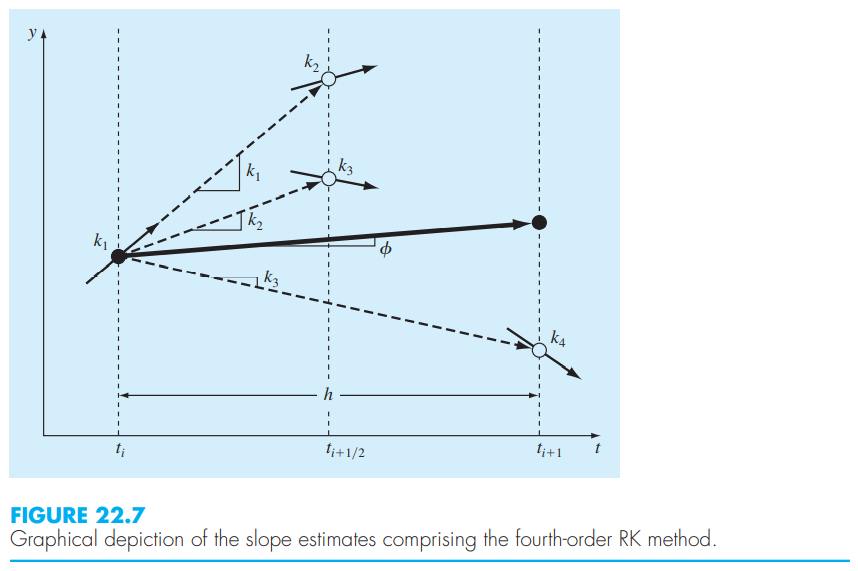
\includegraphics[width=0.85\textwidth]{F22_7}
	\label{F22.7}
\end{figure}\\
 where

\begin{equation}
\tag{22.44a}
k_1 = f(t_i, y_i)
\end{equation}

\begin{equation}
\tag{22.44b}
k_2 = f \left(t_i + \dfrac{1}{2}h, y_i + \dfrac{1}{2} k_1h \right)
\end{equation}

\begin{equation}
\tag{22.44c}
k_3 = f \left(t_i + \dfrac{1}{2}h, y_i + \dfrac{1}{2} k_2h \right)
\end{equation}

\begin{equation}
\tag{22.44d}
k_4 = f(t_i + h, y_i + k_3h)
\end{equation}

Notice that for ODEs that are a function of t alone, the classical fourth-order RK
method is similar to Simpson's 1/3 rule. In addition, the fourth-order RK method is similar to the Heun approach in that multiple estimates of the slope are developed to come up
with an improved average slope for the interval. As depicted in Fig. 22.7, each of the $k$'s represents a slope. Equation (22.44) then represents a weighted average of these to arrive
at the improved slope\\

\vspace{0,3in}
\section{Euler's Method}
\vspace{0,1in}
\hrule
\vspace{0,1in}
\textbf{Problem Statement.} Employ the classical fourth-order RK method to integrate $y' = 4e^{0.8t} - 0.5y$ from $t=0$ to 1 using a step size of 1 with y(0) = 2.

\vspace{0.2in}
\textbf{Solution.}  For this case, the slope at the beginning of the interval is computed as 

$k_1 = f(0,2) = 4e^{0.8(0)} - 0.5(2) = 3$

This value is used to compute a value of y and a slope at the midpoint:

$y(0.5) = 2 + 3(0.5) = 3.5$

$k_2 = f(0.5, 3.5) = 4e^{0.8(0.5) - 0.5(3.5) = 4.217299}$\\
\\
This slope in turn is used to compute another value of y and another slope at the midpoint:

$y(0.5) = 2 + 4.217299(0.5) = 4.108649$

$k_3 = f (0.5, 4.108649) = 4e^{0.8(0.5) − 0.5(4.108649) = 3.912974}$\\
\\
Next, this slope is used to compute a value of y and a slope at the end of the interval:

$y(1.0) = 2 + 3.912974(1.0) = 5.912974$

$k_4 = f (1.0, 5.912974) = 4e^{0.8(1.0) - 0.5(5.912974) = 5.945677}$\\
\\
Finally, the four slope estimates are combined to yield an average slope. This average slope
is then used to make the final prediction at the end of the interval.

$\phi = \dfrac{1}{6} [3 + 2(4.217299) + 2(3.912974) + 5.945677] = 4.201037$

$y(1.0) = 2 + 4.201037(1.0) = 6.201037$\\
\\
which compares favorably with the true solution of 6.194631 ($\varepsilon_{t} = 0.103\%$).
\hrule

\vspace{0.2in}
It is certainly possible to develop fifth- and higher-order RK methods. For example,
Butcher's (1964) fifth-order RK method is written as

\begin{equation}
\tag{22.45}
y_{i+1} = y_i + \dfrac{1}{90}(7k_1 + 32k_3 + 12k_4 + 32k_5 + 7k_6)h
\end{equation}\\
where

\begin{equation}
\tag{22.45a}
k_1 = f(t_i,y_i)
\end{equation}

\begin{equation}
\tag{22.45b}
k_2 = f \left( t_i + \dfrac{1}{4}h, y_i + \dfrac{1}{4}k_1h \right)
\end{equation}

\begin{equation}
\tag{22.45c}
k_3 = f \left(t_i + \dfrac{1}{4}h, y_i + \dfrac{1}{8}k_1h+\dfrac{1}{8}k_2h \right)
\end{equation}

\begin{equation}
\tag{22.45d}
k_4 = f \left(t_i + \dfrac{1}{2}h, y_i - \dfrac{1}{2} k_2h + k_3h \right)
\end{equation}

\begin{equation}
\tag{22.45e}
k_5 = f \left(t_i + \dfrac{3}{4}h, y_i + \dfrac{3}{16}k_1h + \dfrac{9}{16}k_4h \right)
\end{equation}

\begin{equation}
\tag{22.45f}
k_6 = f \left( t_i + h, y_i - \dfrac{3}{7}k_1h + \dfrac{2}{7}k_2h + \dfrac{12}{7}k_3h - \dfrac{12}{7} k_4h + \dfrac{8}{7}k_5h \right)
\end{equation}\\
\\
Note the similarity between Butcher's method and Boole's rule in Table 19.2. As expected,
this method has a global truncation error of $O(h^5)$.

Although the fifth-order version provides more accuracy, notice that six function evaluations are required. Recall that up through the fourth-order versions, n function evaluations are required for an nth-order RK method. Interestingly, for orders higher than four, one or
two additional function evaluations are necessary. Because the function evaluations account
for the most computation time, methods of order five and higher are usually considered relatively less efficient than the fourth-order versions. This is one of the main reasons for the
popularity of the fourth-order RK method.


\vspace{0,6in}
\section{22.5 SYSTEMS OF EQUATIONS}
\vspace{0,1in}
\hrule
\vspace{0,1in}

Many practical problems in engineering and science require the solution of a system of simultaneous ordinary differential equations rather than a single equation. Such systems may
be represented generally as

$$\dfrac{dy_1}{dt} = f_1(t,y_1,y_2, \cdots , y_n)$$
\begin{equation}
\tag{22.46}
\dfrac{dy_2}{dt} = f_2(t,y_1,y_2, \cdots, y_n)
\end{equation}
$$\vdots$$
$$\dfrac{dy_n}{dt} = f_n(t,y_1,y_2, \cdots , y_n)$$\\
The solution of such a system requires that n initial conditions be known at the starting
value of t.

An example is the calculation of the bungee jumper's velocity and position that we set
up at the beginning of this chapter. For the free-fall portion of the jump, this problem
amounts to solving the following system of ODEs:

\begin{equation}
\tag{22.47}
\dfrac{dx}{dt} = v
\end{equation}

\begin{equation}
\tag{22.48}
\dfrac{dv}{dt} = g - \dfrac{c_{d}}{m}v^2
\end{equation}\\
\\
If the stationary platform from which the jumper launches is defined as x = 0, the initial
conditions would be x(0) = v(0) = 0.

\subsection{ Euler's Method}

All the methods discussed in this chapter for single equations can be extended to systems
of ODEs. Engineering applications can involve thousands of simultaneous equations. In
each case, the procedure for solving a system of equations simply involves applying the
one-step technique for every equation at each step before proceeding to the next step. This
is best illustrated by the following example for Euler's method.


\vspace{0,3in}
\section{Euler's Method}
\vspace{0,1in}
\hrule
\vspace{0,1in}
\textbf{Problem Statement.} Solve for the velocity and position of the free-falling bungee jumper
using Euler's method. Assuming that at t = 0, x = v = 0, and integrate to t = 10 s with a
step size of 2 s. As was done previously in Examples 1.1 and 1.2, the gravitational acceleration is $9.81 m/s^2$, and the jumper has a mass of 68.1 kg with a drag coefficient of 0.25 kg/m. 

Recall that the analytical solution for velocity is [Eq. (1.9)]:

$v(t) = \sqrt{\dfrac{gm}{c_{d}}} tanh \left( \sqrt{\dfrac{gc_d}{m}}t \right)$\\
\\
This result can be substituted into Eq. (22.47) which can be integrated to determine an
analytical solution for distance as

$x(t) = \dfrac{m}{c_d} ln \left[ cosh \left( \sqrt{\dfrac{gc_d}{m}}t \right) \right]$\\
\\
Use these analytical solutions to compute the true relative errors of the results.

\vspace{0.2in}
\textbf{Solution.} The ODEs can be used to compute the slopes at $t$ = 0 as

$\dfrac{dx}{dt} = 0$

$\dfrac{dv}{dt} = 9.81 - \dfrac{0.25}{68.1} (0)^2 = 9.81$\\
\\
Euler's method is then used to compute the values at t = 2 s,

$x = 0 + 0(2) = 0$

$v = 0 + 9.81(2) = 19.62$\\
\\
The analytical solutions can be computed as x(2) = 19.16629 and v(2) = 18.72919. Thus,
the percent relative errors are 100\% and 4.756\%, respectively.

The process can be repeated to compute the results at t = 4 as

$x = 0 + 19.62(2) = 39.24$

$v = 19.62 + \left( 9.81 − \dfrac{0.25}{68.1} (19.62)^2 \right)2 = 36.41368$\\
\\
Proceeding in a like manner gives the results displayed in Table 22.3.

\textbf{Table 22.3} Distance and velocity of a free-falling bungee jumper as computed
numerically with Euler's method.\\

\begin{tabular}{lcccccc}
\hline

	\textbf{$t$} \; \; \; \; \; & \textbf{$x_{true}$} \; \; \; \; \; & \textbf{$v_{true}$} \; \; \; \; \; & \textbf{$x_{Euler}$} \; \; \; \; \; & \textbf{$v_Euler$} \; \; \; \; \; & \textbf{$\varepsilon_{t}(x)$} \; \; \; \; \; & \textbf{$\varepsilon_{t}(v)$}\\
	
\hline

	0 & 0 & 0 & 0 & 0 & \vspace{0in} & \vspace{0in}\\
	
	2 & 19.1663 & 18.7292 & 0 & 19.6200 & 100.00\% & 4.76\%\\
	
	4 & 71.9304 & 33.1118 & 39.2400 & 36.4137 & 45.45\% & 9.97\%\\
	
	6 & 147.9462 & 42.0762 & 112.0674 & 46.2983 & 24.25\% & 10.03\%\\
	
	8 & 237.5104 & 46.9575 & 204.6640 & 50.1802 & 13.83\% & 6.86\%\\
	
	10 & 334.1782 & 49.4214 & 305.0244 & 51.3123 & 8.72\% & 3.83\%\\

\hline
\end{tabular}\\
\\
\\
\hrule
\vspace{0.2in}
Although the foregoing example illustrates how Euler's method can be implemented for
systems of ODEs, the results are not very accurate because of the large step size. In addition,
the results for distance are a bit unsatisfying because x does not change until the second
iteration. Using a much smaller step greatly mitigates these deficiencies. As described next,
using a higher-order solver provides decent results even with a relatively large step size.

\subsection{Runge-Kutta Methods}

Note that any of the higher-order RK methods in this chapter can be applied to systems of
equations. However, care must be taken in determining the slopes. Figure 22.7 is helpful in
visualizing the proper way to do this for the fourth-order method. That is, we first develop
slopes for all variables at the initial value. These slopes (a set of $k_1$'s) are then used to make
predictions of the dependent variable at the midpoint of the interval. These midpoint values are in turn used to compute a set of slopes at the midpoint (the $k_2$'s). These new slopes
are then taken back to the starting point to make another set of midpoint predictions that
lead to new slope predictions at the midpoint (the $k_3$'s). These are then employed to make
predictions at the end of the interval that are used to develop slopes at the end of the interval (the $k_4$'s). Finally, the k's are combined into a set of increment functions [as in
Eq. (22.44)] that are brought back to the beginning to make the final predictions. The following example illustrates the approach.

\vspace{0,3in}
\section{Solving Systems of ODEs with the Fourth-Order RK Method}
\vspace{0,1in}
\hrule
\vspace{0,1in}
\textbf{Problem Statement.} Use the fourth-order RK method to solve for the same problem we
addressed in Example 22.4.
\vspace{0.2in}\\
\textbf{Solution.} First, it is convenient to express the ODEs in the functional format of
Eq. (22.46) as

$\dfrac{dx}{dt} = f_1(t,x,v) = v$

$\dfrac{dv}{dt} = f_2(t,x,v) = g - \dfrac{c_d}{m} v^2$\\
\\
The first step in obtaining the solution is to solve for all the slopes at the beginning of the
interval:

$k_{1,1} = f_1(0,0,0) = 0$

$k_{1,2} = f_2(0,0,0) = 9.81 - \dfrac{0.25}{68.1}(0)^2 = 9.81$\\
\\
where $k_{i,j}$ is the ith value of k for the jth dependent variable. Next, we must calculate the
first values of x and v at the midpoint of the first step:

$x(1) = x(0) + k_{1,1}\dfrac{h}{2} = 0 + 0\dfrac{2}{2} = 0$

$v(1) = v(0) + k_{1,2} \dfrac{h}{2} = 0 + 9.81\dfrac{2}{2} = 9.81$\\
\\
which can be used to compute the first set of midpoint slopes:

$k_{2,1} = f_1(1,0,9.81) = 9.8100$

$k_{2,2} = f_2(1,0,9.81) = 9.4567$\\
\\
These are used to determine the second set of midpoint predictions:

$x(1) = x(0) + k_{2,1} \dfrac{h}{2} = 0 + 9.8100 \dfrac{2}{2} = 9.8100$

$v(1) = v(0) + k_{2,2} \dfrac{h}{2} = 0 + 9.4567 \dfrac{2}{2} = 9.4567$\\
\\
which can be used to compute the second set of midpoint slopes:

$k_{3,1} = f_1(1, 9.8100, 9.4567) = 9.4567$

$k_{3,2} = f_2(1, 9.8100, 9.4567) = 9.4817$\\
\\
These are used to determine the predictions at the end of the interval:

$x(2) = x(0) + k_{3,1}h = 0 + 9.4567(2) = 18.9134$

$v(2) = v(0) + k_{3,2}h = 0 + 9.4817(2) = 18.9634$\\
\\
which can be used to compute the endpoint slopes:

$k_{4,1} = f_1(2, 18.9134, 18.9634) = 18.9634$

$k_{4,2} = f_2(2, 18.9134, 18.9634) = 8.4898$\\
\\
The values of k can then be used to compute [Eq. (22.44)]:\\

$ x(2) = 0 + \dfrac{1}{6} [0 + 2(9.8100 + 9.4567) + 18.9634] 2 = 19.1656$\\

$ v(2) = 0 + \dfrac{1}{6} [9.8100 + 2(9.4567 + 9.4817) + 8.4898] 2 = 18.7256$\\

Proceeding in a like manner for the remaining steps yields the values displayed in
Table 22.4. In contrast to the results obtained with Euler's method, the fourth-order RK
predictions are much closer to the true values. Further, a highly accurate, nonzero value is
computed for distance on the first step.

\vspace{0,3in}
\textbf{Table 22.4} Distance and velocity of a free-falling bungee jumper as computed
numerically with the fourth-order RK method.
\\
\begin{tabular}{lcccccc}
\hline

	\textbf{$t$} \; \; \; \; \; & \textbf{$x_{true}$} 
	\textbf{$t$} \; \; \; \; \; & \textbf{$v_{true}$} 
	\textbf{$t$} \; \; \; \; \; & \textbf{$X_{RK4}$} 
	\textbf{$t$} \; \; \; \; \; & \textbf{$V_{RK4}$} 
	\textbf{$t$} \; \; \; \; \; & \textbf{$\varepsilon_{t}(X)$} 
	\textbf{$t$} \; \; \; \; \; & \textbf{$\varepsilon_{t}(V)$}\\
	
\hline

	0 & 0 & 0 & 0 & 0 & \vspace{0in} & \vspace{0in}\\

	2 & 19.1663 & 18.7292 & 19.1656 & 18.7256 & 0.004\% & 0.019\%\\

	4 & 71.9304 & 33.1118 & 71.9311 & 33.0995 & 0.001\% & 0.037\%\\

	6 & 147.9462 & 42.0762 & 147.9521 & 42.0547 & 0.004\% & 0.051\%\\

	8 & 237.5104 & 46.9575 & 237.5104 & 46.9345 & 0.000\% & 0.049\%\\

	10 & 334.1782 & 49.4214 & 334.1626 & 49.4027 & 0.005\% & 0.038\%\\


\hline
\end{tabular}

\subsection{MATLAB M-file Function: \texttt{rk4sys}}
\vspace{0.1 in}
Figure 22.8 shows an M-file called rk4sys that uses the fourth-order Runge-Kutta method
to solve a system of ODEs. This code is similar in many ways to the function developed
earlier (Fig. 22.3) to solve a single ODE with Euler's method. For example, it is passed the
function name defining the ODEs through its argument.

\begin{figure}[hbt!]
	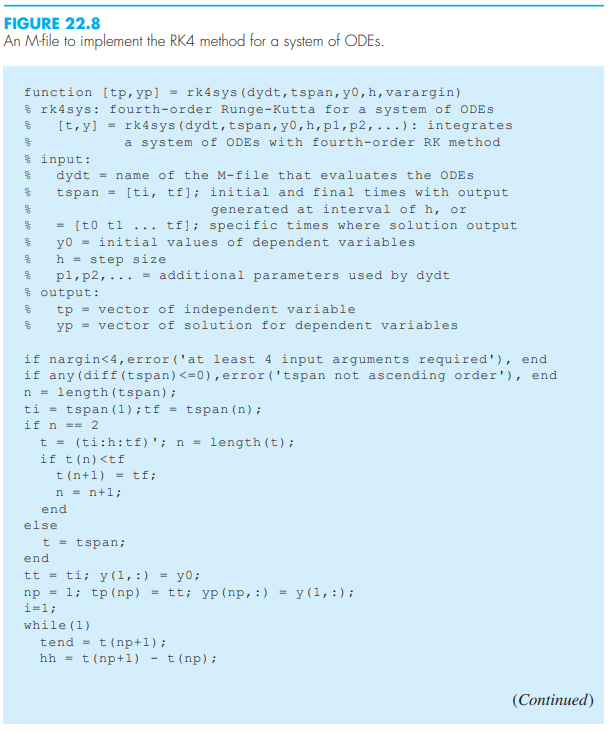
\includegraphics[width=0.75\textwidth]{F22_8_1}
	\label{F22.8.1}
\end{figure}

\begin{figure}[hbt!]
	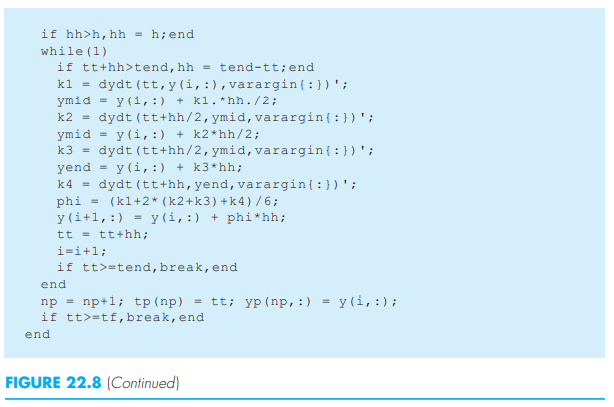
\includegraphics[width=0.75\textwidth]{F22_8_2}
	\label{F22.8.2}
\end{figure}

However, it has an additional feature that allows you to generate output in two ways,
depending on how the input variable \texttt{tspan} is specified. As was the case for Fig. 22.3, you
can set \texttt{tspan = [ti tf]}, where \texttt{ti} and \texttt{tf} are the initial and final times, respectively.
If done in this way, the routine automatically generates output values between these limits
at equal spaced intervals h. Alternatively, if you want to obtain results at specific times, you
can define \texttt{tspan = [t0,t1,...,tf]}. Note that in both cases, the \texttt{tspan} values must
be in ascending order.
We can employ \texttt{rk4sys} to solve the same problem as in Example 22.5. First, we can
develop an M-file to hold the ODEs:

\begin{verbatim}
   function dy = dydtsys(t, y)
   dy = [y(2);9.81-0.25/68.1*y(2)^2];
\end{verbatim}

where \texttt{y(1)} = distance ($x$) and \texttt{y(2)} = velocity ($v$). The solution can then be generated as

\begin{verbatim}
   >> [t y] = rk4sys(@dydtsys,[0 10],[0 0],2);
   >> disp([t' y(:,1) y(:,2)])
   
           0          0          0
      2.0000    19.1656    18.7256
      4.0000    71.9311    33.0995
      6.0000   147.9521    42.0547
      8.0000   237.5104    46.9345
     10.0000   334.1626    49.4027
\end{verbatim}

We can also use \texttt{tspan} to generate results at specific values of the independent variable. For example,

\begin{verbatim}
   >> tspan=[0 6 10];
   >> [t y] = rk4sys(@dydtsys,tspan,[0 0],2);
   >> disp([t' y(:,1) y(:,2)])

            0           0          0
       6.0000    147.9521    42.0547
      10.0000    334.1626    49.4027
\end{verbatim}

\subsection{Case Study: Predator-Prey Models and Chaos}

\noindent\textbf{Background}. Engineers and scientists deal with a variety of problems involving systems of nonlinear ordinary differential equations. This case study focuses on two of these
applications. The first relates to predator-prey models that are used to study species interactions. The second are equations derived from fluid dynamics that are used to simulate the
atmosphere.

\textit{Predator-prey models} were developed independently in the early part of the twentieth
century by the Italian mathematician Vito Volterra and the American biologist Alfred
Lotka. These equations are commonly called \textit{Lotka-Volterra equations}. The simplest version is the following pairs of ODEs:

\begin{equation}
    \tag{22.49}
    \frac{dx}{dt}=ax-bxy
\end{equation}

\begin{equation}
    \tag{22.50}
    \frac{dy}{dt}=-cy+dxy
\end{equation}

\noindent where $x$ and $y=$ the number of prey and predators, respectively, $a=$ the prey growth rate, $c=$ the predator death rate, and $b$ and $d=$ the rates characterizing the effect of the predatorprey interactions on the prey death and the predator growth, respectively. The multiplicative terms (i.e., those involving $x y$ ) are what make such equations nonlinear.

An example of a simple nonlinear model based on atmospheric fluid dynamics is the \textit{Lorenz equations} created by the American meteorologist Edward Lorenz:
$$
\begin{aligned}
&\frac{d x}{d t}=-\sigma x-\sigma y \\
&\frac{d y}{d t}=r x-y-x z \\
&\frac{d z}{d t}=-b z+x y
\end{aligned}
$$
Lorenz developed these equations to relate the intensity of atmospheric fluid motion $x$ to temperature variations $y$ and $z$ in the horizontal and vertical directions, respectively. As with the predator-prey model, the nonlinearities stem from the simple multiplicative terms: $xz$ and $xy$.

Use numerical methods to obtain solutions for these equations. Plot the results to visualize how the dependent variables change temporally. In addition, graph the dependent variables versus each other to see whether any interesting patterns emerge.

\noindent\textbf{Solution.} The following parameter values can be used for the predator-prey simulation: $a = 1.2,\ b = 0.6,\ c = 0.8$, and $d = 0.3$. Employ initial conditions of $x = 2$ and $y = 1$ and integrate from $t = 0$ to 30, using a step size of $h = 0.0625$.

First, we can develop a function to hold the differential equations:\vspace{\smallskipamount}

\noindent\texttt{function yp = predprey(t,y,a,b,c,d)\\
yp = [a*y(1)-b*y(1)*y(2);-c*y(2)+d*y(1)*y(2)];}\vspace{\medskipamount}

The following script employs this function to generate solutions with both the Euler
and the fourth-order RK methods. Note that the function \texttt{eulersys} was based on modifying the \texttt{rk4sys} function (Fig. 22.8). We will leave the development of such an M-file as a
homework problem. In addition to displaying the solution as a time-series plot ($x$ and $y$
versus $t$), the script also generates a plot of $y$ versus $x$. Such \textit{phase-plane} plots are often
useful in elucidating features of the model's underlying structure that may not be evident
from the time series.\vspace{\medskipamount}

\noindent\texttt{h=0.0625;tspan=[0 40];y0=[2 1];\\
a=1.2;b=0.6;c=0.8;d=0.3;\\}
\noindent\texttt{[t y] = eulersys(@predprey,tspan,y0,h,a,b,c,d);\\}
\noindent\texttt{subplot(2,2,1);plot(t,y(:,1),t,y(:,2),'--')\\
legend('prey','predator');title('(a) Euler time plot')\\
subplot(2,2,2);plot(y(:,1),y(:,2))\\
title('(b) Euler phase plane plot')\\}
\noindent\texttt{[t y] = rk4sys(@predprey,tspan,y0,h,a,b,c,d);\\}
\noindent\texttt{subplot(2,2,3);plot(t,y(:,1),t,y(:,2),'--')\\
title('(c) RK4 time plot')\\
subplot(2,2,4);plot(y(:,1),y(:,2))\\
title('(d) RK4 phase plane plot')}\vspace{\smallskipamount}

The solution obtained with Euler's method is shown at the top of Fig. 22.9. The time
series (Fig. 22.9$a$) indicates that the amplitudes of the oscillations are expanding. This is
reinforced by the phase-plane plot (Fig. 22.9$b$). Hence, these results indicate that the crude
Euler method would require a much smaller time step to obtain accurate results.

In contrast, because of its much smaller truncation error, the RK4 method yields good results with the same time step. As in Fig. 22.9$c$, a cyclical pattern emerges in time. Because the
predator population is initially small, the prey grows exponentially. At a certain point, the
prey become so numerous that the predator population begins to grow. Eventually, the increased predators cause the prey to decline. This decrease, in turn, leads to a decrease of the
predators. Eventually, the process repeats. Notice that, as expected, the predator peak lags the
prey. Also, observe that the process has a fixed period-that is, it repeats in a set time.

\begin{figure}[H]
    \centering
    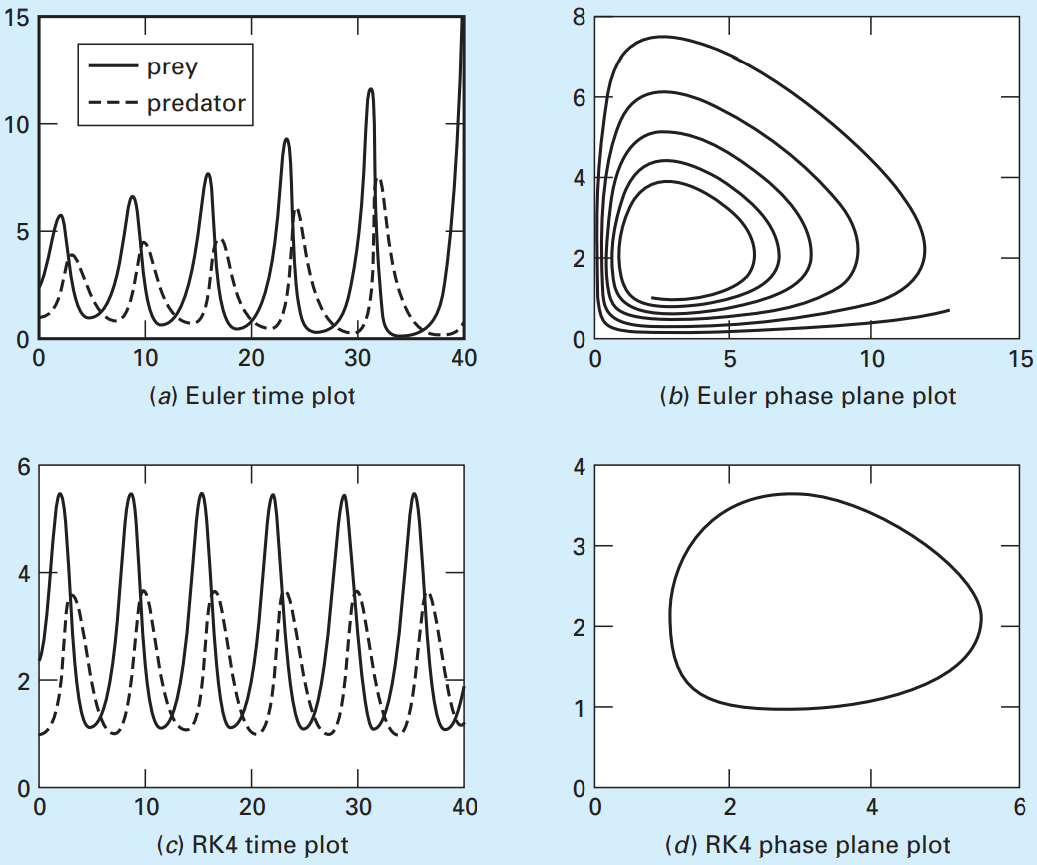
\includegraphics[scale=0.4]{fig_22_9}
   \caption{\textsf{Solution for the Lotka-Volterra model. Euler;s method (a) time-series and (b) phase-plane plots, and
   RK4 method (c) time-series and (d) phase-plane plots.}}\label{fig:fig_22_9}
\end{figure}

The phase-plane representation for the accurate $\mathrm{RK} 4$ solution (Fig. $22.9 d$ ) indicates that the interaction between the predator and the prey amounts to a closed counterclockwise orbit. Interestingly, there is a resting or \textit{critical point} at the center of the orbit.
The exact location of this point can be determined by setting Eqs. (22.49) and (22.50) to steady state $(d y / d t=d x / d t=0)$ and solving for $(x, y)=(0,0)$ and $(c / d, a / b)$. The former is the trivial result that if we start with neither predators nor prey, nothing will happen. The latter is the more interesting outcome that if the initial conditions are set at $x=c / d$ and $y=a / b$, the derivatives will be zero, and the populations will remain constant.

Now, let's use the same approach to investigate the trajectories of the Lorenz equations with the following parameter values: $a=10, b=8 / 3$, and $r=28$. Employ initial conditions of $x=y=z=5$ and integrate from $t=0$ to 20 . For this case, we will use the fourth-order $\mathrm{RK}$ method to obtain solutions with a constant time step of $h=0.03125$.

\begin{figure}[H]
    \centering
    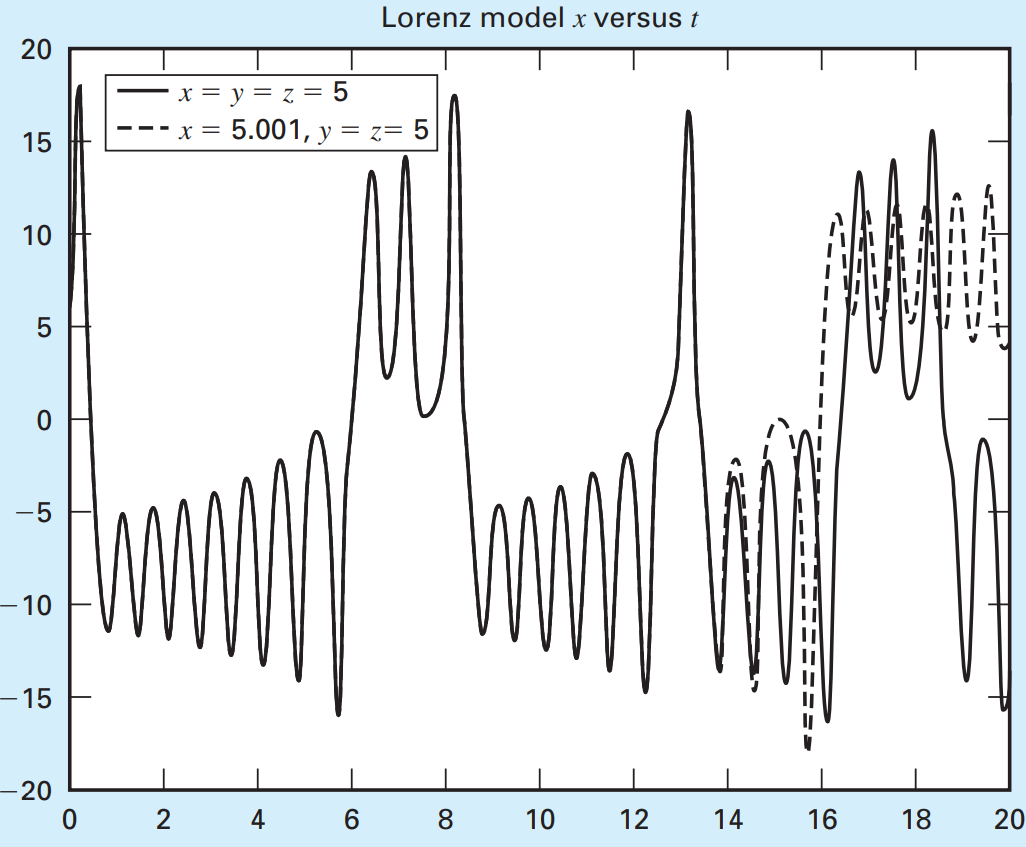
\includegraphics[scale=0.35]{fig_22_10}
   \caption{\textsf{Time-domain representation of $x$ versus $t$ for the Lorenz equations. The solid time series is for the initial conditions (5, 5, 5). The dashed line is where the initial condition for $x$ is perturbed slightly
   (5.001, 5, 5).}}\label{fig:fig_22_10}
\end{figure}

The results are quite different from the behavior of the Lotka-Volterra equations. As in
Fig. 22.10, the variable $x$ seems to be undergoing an almost random pattern of oscillations,
bouncing around from negative values to positive values. The other variables exhibit
similar behavior. However, even though the patterns seem random, the frequency of the
oscillation and the amplitudes seem fairly consistent.

An interesting feature of such solutions can be illustrated by changing the initial condition for x slightly (from 5 to 5.001). The results are superimposed as the dashed line in
Fig. 22.10. Although the solutions track on each other for a time, after about $t = 15$ they
diverge significantly. Thus, we can see that the Lorenz equations are quite sensitive to
their initial conditions. The term \textit{chaotic} is used to describe such solutions. In his original study, this led Lorenz to the conclusion that long-range weather forecasts might be
impossible!

The sensitivity of a dynamical system to small perturbations of its initial conditions is
sometimes called the \textit{butterfly effect}. The idea is that the flapping of a butterfly's wings
might induce tiny changes in the atmosphere that ultimately leads to a large-scale weather
phenomenon like a tornado.

\begin{figure}[H]
    \centering
    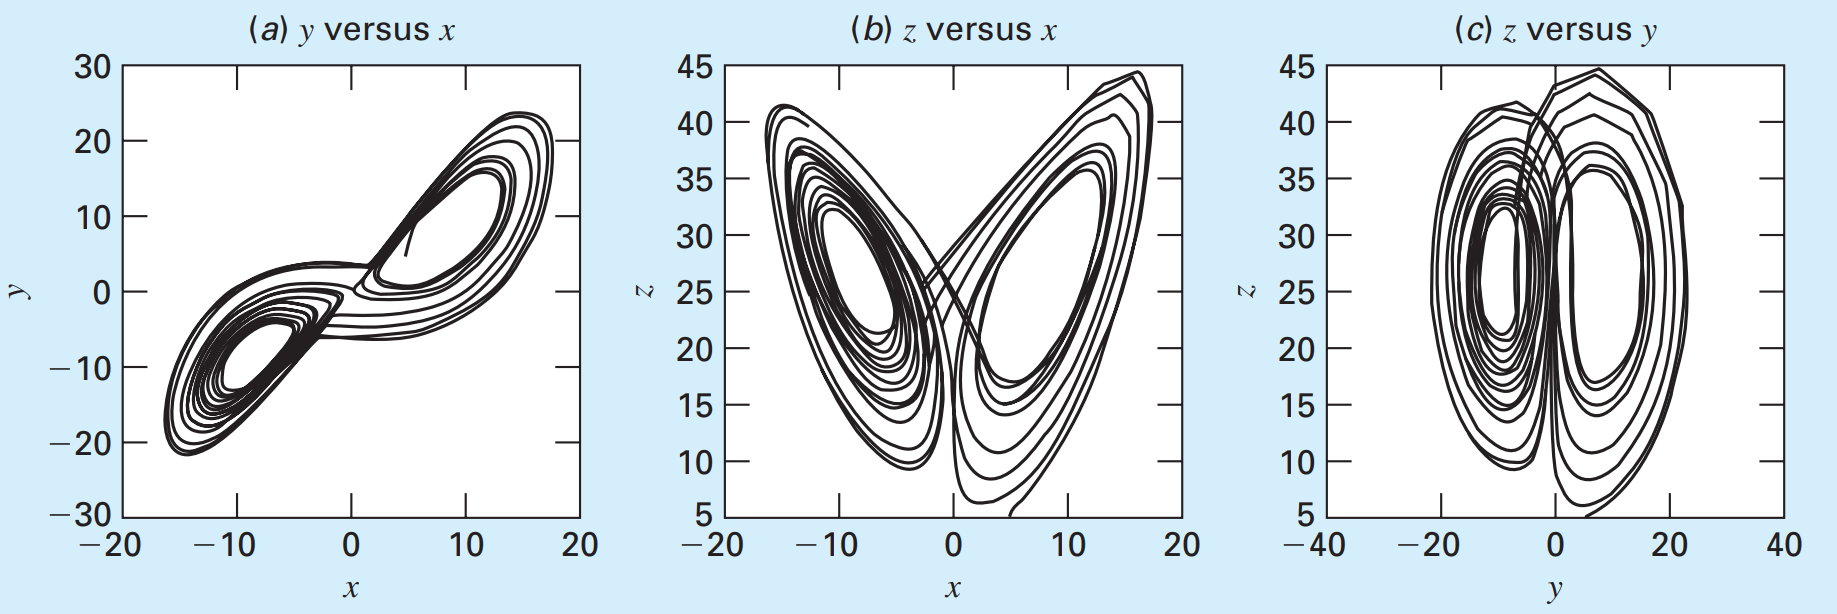
\includegraphics[scale=0.35]{fig_22_11}
   \caption{\textsf{Phase-plane representation for the Lorenz equations. (a) xy, (b) xz, and (c) yz projections.}}\label{fig:fig_22_11}
\end{figure}

Although the time-series plots are chaotic, phase-plane plots reveal an underlying
structure. Because we are dealing with three independent variables, we can generate
projections. Figure 22.11 shows projections in the $xy$, $xz$, and the $yz$ planes. Notice how a
structure is manifest when perceived from the phase-plane perspective. The solution forms
orbits around what appear to be critical points. These points are called \textit{strange attractors} in
the jargon of mathematicians who study such nonlinear systems.

Beyond the two-variable projections, MATLAB's \texttt{plot3} function provides a vehicle
to directly generate a three-dimensional phase-plane plot:\vspace{\medskipamount}

\noindent\texttt{>> plot3(y(:,1),y(:,2),y(:,2))\\
>> xlabel('x');ylabel('y');zlabel('z');grid}\vspace{\medskipamount}

\noindent As was the case for Fig. 22.11, the three-dimensional plot (Fig 22.12) depicts trajectories
cycling in a definite pattern around a pair of critical points.

As a final note, the sensitivity of chaotic systems to initial conditions has implications
for numerical computations. Beyond the initial conditions themselves, different step sizes
or different algorithms (and in some cases, even different computers) can introduce small
differences in the solutions. In a similar fashion to Fig. 22.10, these discrepancies will
eventually lead to large deviations. Some of the problems in this chapter and in Chap. 23
are designed to demonstrate this issue.

\begin{figure}[H]
    \centering
    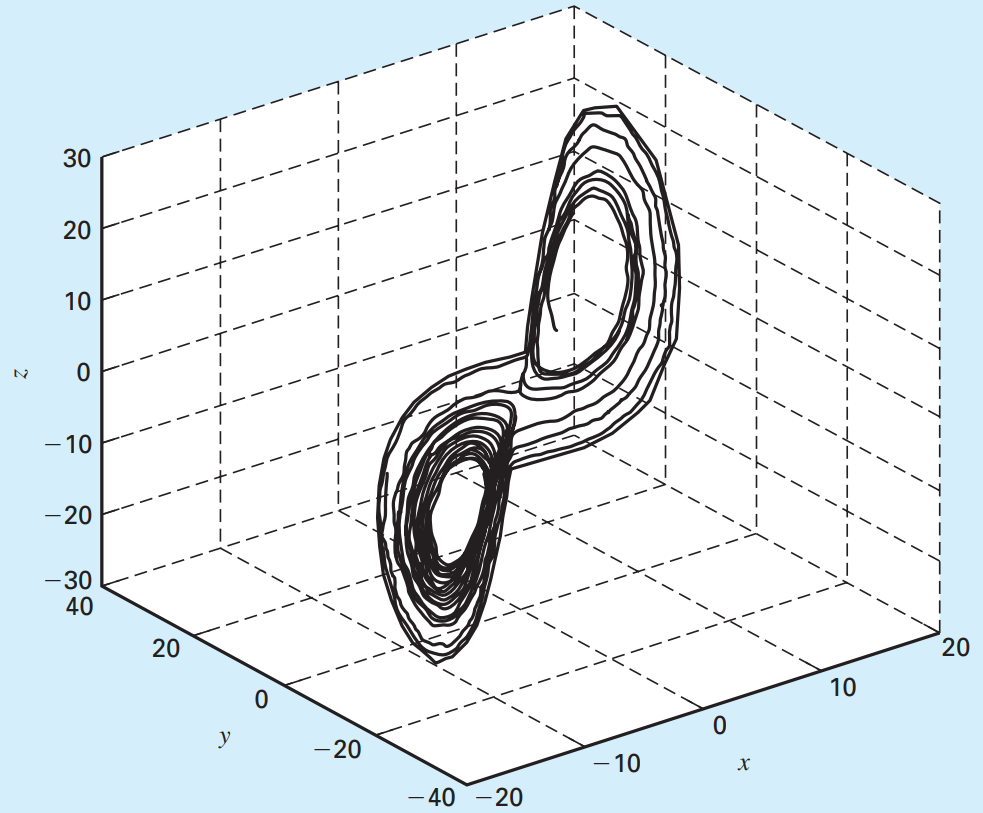
\includegraphics[scale=0.4]{fig_22_12}
   \caption{\textsf{Three-dimensional phase-plane representation for the Lorenz equations generated with MATLAB's \texttt{plot3} function.}}\label{fig:fig_22_12}
\end{figure}\vspace{2cm}


\subsection{Problems}

\begin{multicols}{2}

    \noindent\textbf{22.1} Solve the following initial value problem over the interval from $t=0$ to 2 where $y(0)=1$. Display all your results on the same graph.
    $$
    \frac{d y}{d t}=y t^{3}-1.5 y
    $$
    \textbf{(a)} Analytically.\\
    \textbf{(b)} Using Euler's method with $h=0.5$ and $0.25$.\\
    \textbf{(c)} Using the midpoint method with $h=0.5$.\\
    \textbf{(d)} Using the fourth-order RK method with $h=0.5$.\vspace{2mm}

    \noindent\textbf{22.2} Solve the following problem over the interval from $x=0$ to 1 using a step size of $0.25$ where $y(0)=1$. Display all your results on the same graph.
    $$
    \frac{d y}{d x}=(1+4 x) \sqrt{y}
    $$
    \textbf{(a)} Analytically.\\
    \textbf{(b)} Using Euler's method.\\
    \textbf{(c)} Using Heun's method without iteration.\\
    \textbf{(d)} Using Ralston's method.\\
    \textbf{(e)} Using the fourth-order RK method.\vspace{2mm}

    \noindent\textbf{22.3} Solve the following problem over the interval from $t=0$ to 2 using a step size of $0.5$ where $y(0)=1$. Display all your results on the same graph.
    $$
    \frac{d y}{d t}=-2 y+t^{2}
    $$
    Obtain your solutions with \textbf{(a)} Heun's method without iterating the corrector, \textbf{(b)} Heun's method with iterating the corrector until $\varepsilon_{s}<0.1 \%$, \textbf{(c)} the midpoint method, and \textbf{(d)}Ralston's method.\vspace{2mm}

    \noindent\textbf{22.4} The growth of populations of organisms has many engineering and scientific applications. One of the simplest models assumes that the rate of change of the population $p$ is proportional to the existing population at any time $t$ :
    \begin{equation}
        \tag{P22.4.1}
        \frac{d p}{d t}=k_{g} p
    \end{equation}
    
    \noindent where $k_{g}=$ the growth rate. The world population in millions from 1950 through 2000 was
    
    \begin{figure}[H]
        \centering
        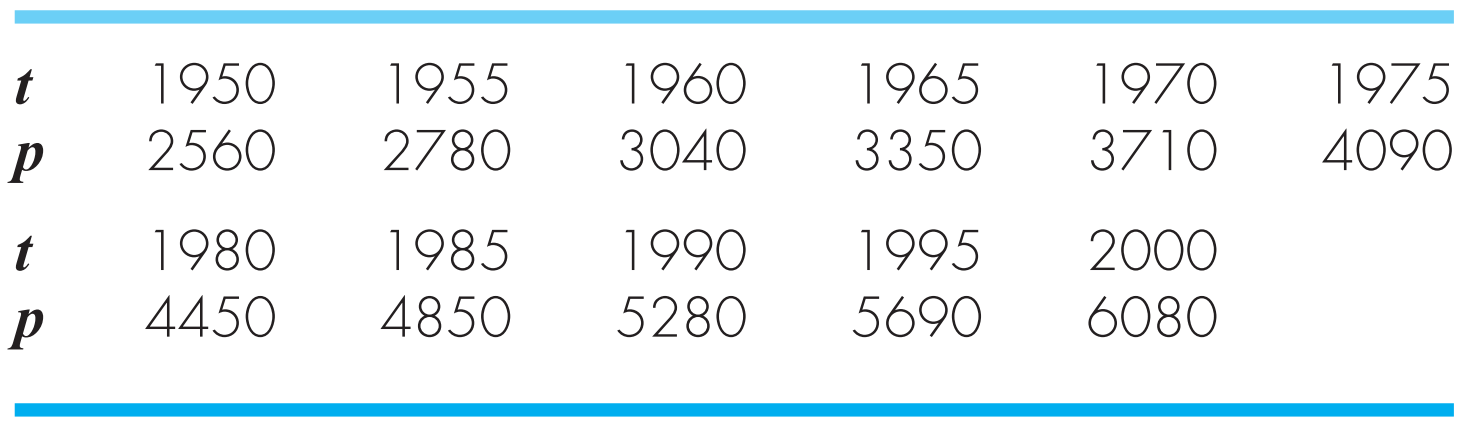
\includegraphics[scale=0.25]{fig_P_22_4}
    \end{figure}
    
    \noindent\textbf{(a)} Assuming that Eq. (P22.4.1) holds, use the data from
    1950 through 1970 to estimate $k_g$.\\
    \textbf{(b)} Use the fourth-order RK method along with the results of \textbf{(a)} to stimulate the world population from 1950 to 2050 with a step size of 5 years. Display your simulation results along with the data on a plot.\vspace{2mm}

    \noindent\textbf{22.5} Although the model in Prob. $22.4$ works adequately when population growth is unlimited, it breaks down when factors such as food shortages, pollution, and lack of space inhibit growth. In such cases, the growth rate is not a constant, but can be formulated as
    $$
    k_{g}=k_{g m}\left(1-p / p_{\max }\right)
    $$
    where $k_{g m}=$ the maximum growth rate under unlimited conditions, $p=$ population, and $p_{\max }=$ the maximum population. Note that $p_{\max }$ is sometimes called the carrying capacity. Thus, at low population density $p \ll p_{\max }$, $k_{g} \rightarrow k_{g m}$. As $p$ approaches $p_{\max }$, the growth rate approaches zero. Using this growth rate formulation, the rate of change of population can be modeled as
    $$
    \frac{d p}{d t}=k_{g m}\left(1-p / p_{\max }\right) p
    $$ This is referred to as the logistic model. The analytical solution to this model is
    $$
    p=p_{0} \frac{p_{\max }}{p_{0}+\left(p_{\max }-p_{0}\right) e^{-k_{g m} t}}
    $$
    Simulate the world's population from 1950 to 2050 using \textbf{(a)} the analytical solution, and \textbf{(b)} the fourth-order RK method with a step size of 5 years. Employ the following initial conditions and parameter values for your simulation: $p_{0}($ in 1950$)=2,560$ million people, $k_{g m}=0.026 / \mathrm{yr}$, and $p_{\max }=12,000$ million people. Display your results as a plot along with the data from Prob. 22.4.\vspace{2mm}

    \noindent\textbf{22.6} Suppose that a projectile is launched upward from the earth's surface. Assume that the only force acting on the object is the downward force of gravity. Under these conditions, a force balance can be used to derive
    $$
    \frac{d v}{d t}=-g(0) \frac{R^{2}}{(R+x)^{2}}
    $$
    where $v=$ upward velocity $(\mathrm{m} / \mathrm{s}), t=$ time $(\mathrm{s}), x=$ altitude (m) measured upward from the earth's surface, $g(0)=$ the gravitational acceleration at the earth's surface $\left(\cong 9.81 \mathrm{~m} / \mathrm{s}^{2}\right)$, and $R=$ the earth's radius $(\cong 6.37 \times$ $\left.10^{6} \mathrm{~m}\right)$. Recognizing that $d x / d t=v$, use Euler's method to determine the maximum height that would be obtained if $v(t=0)=1500 \mathrm{~m} / \mathrm{s}$.\vspace{2mm}

    \noindent\textbf{22.7} Solve the following pair of ODEs over the interval from $t=0$ to $0.4$ using a step size of $0.1$. The initial conditions are $y(0)=2$ and $z(0)=4$. Obtain your solution with \textbf{(a)} Euler's method and \textbf{(b)} the fourth-order RK method. Display your results as a plot.
    $$
    \begin{aligned}
    &\frac{d y}{d t}=-2 y+5 e^{-t} \\
    &\frac{d z}{d t}=-\frac{y z^{2}}{2}
    \end{aligned}
    $$\vspace{2mm}

    \noindent\textbf{22.8} The van der Pol equation is a model of an electronic circuit that arose back in the days of vacuum tubes:
    $$
    \frac{d^{2} y}{d t^{2}}-\left(1-y^{2}\right) \frac{d y}{d t}+y=0
    $$
    Given the initial conditions, $y(0)=y^{\prime}(0)=1$, solve this equation from $t=0$ to 10 using Euler's method with a step size of \textbf{(a)} $0.25$ and \textbf{(b)} $0.125$. Plot both solutions on the same graph.\vspace{2mm}

    \noindent\textbf{22.9} 22.9 Given the initial conditions, $y(0)=1$ and $y^{\prime}(0)=0$, solve the following initial-value problem from $t=0$ to 4:
    $$
    \frac{d^{2} y}{d t^{2}}+4 y=0
    $$ Obtain your solutions with \textbf{(a)} Euler's method and \textbf{(b)} the fourth-order $R K$ method. In both cases, use a step size of $0.1$. Plot both solutions on the same graph along with the exact solution $y=\cos 2 t$.\vspace{2mm}

    \noindent\textbf{22.10} Develop an M-file to solve a single ODE with Heun's
    method with iteration. Design the M-file so that it creates a
    plot of the results. Test your program by using it to solve for
    population as described in Prob. 22.5. Employ a step size of
    5 years and iterate the corrector until $\epsilon_s < 0.1\%$.\vspace{2mm}

    \noindent\textbf{22.11} Develop an M-file to solve a single ODE with the
    midpoint method. Design the M-file so that it creates a plot
    of the results. Test your program by using it to solve for population as described in Prob. 22.5. Employ a step size of
    5 years.\vspace{2mm}

    \noindent\textbf{22.12} Develop an M-file to solve a single ODE with the
    fourth-order RK method. Design the M-file so that it creates
    a plot of the results. Test your program by using it to solve
    Prob. 22.2. Employ a step size of 0.1.\vspace{2mm}

    \noindent\textbf{22.13} Develop an M-file to solve a system of ODEs with
    Euler's method. Design the M-file so that it creates a plot of
    the results. Test your program by using it to solve Prob. 22.7
    with a step size of 0.25\vspace{2mm}

    \noindent\textbf{22.14} Isle Royale National Park is a 210-square-mile archipelago composed of a single large island and many small
    islands in Lake Superior. Moose arrived around 1900, and
    by 1930, their population approached 3000, ravaging vegetation. In 1949, wolves crossed an ice bridge from Ontario.
    Since the late 1950s, the numbers of the moose and wolves
    have been tracked.\\
    \textbf{(a)} Integrate the Lotka-Volterra equations (Sec. 22.6) from 1960 through 2020 using the following coefficient values: $a=0.23, b=0.0133, c=0.4$, and $d=0.0004$. Compare your simulation with the data using a timeseries plot and determine the sum of the squares of the residuals between your model and the data for both the moose and the wolves.
    \textbf{(b)} Develop a phase-plane plot of your solution.\vspace{2mm}

    \end{multicols}

    \begin{figure}[H]
        \centering
        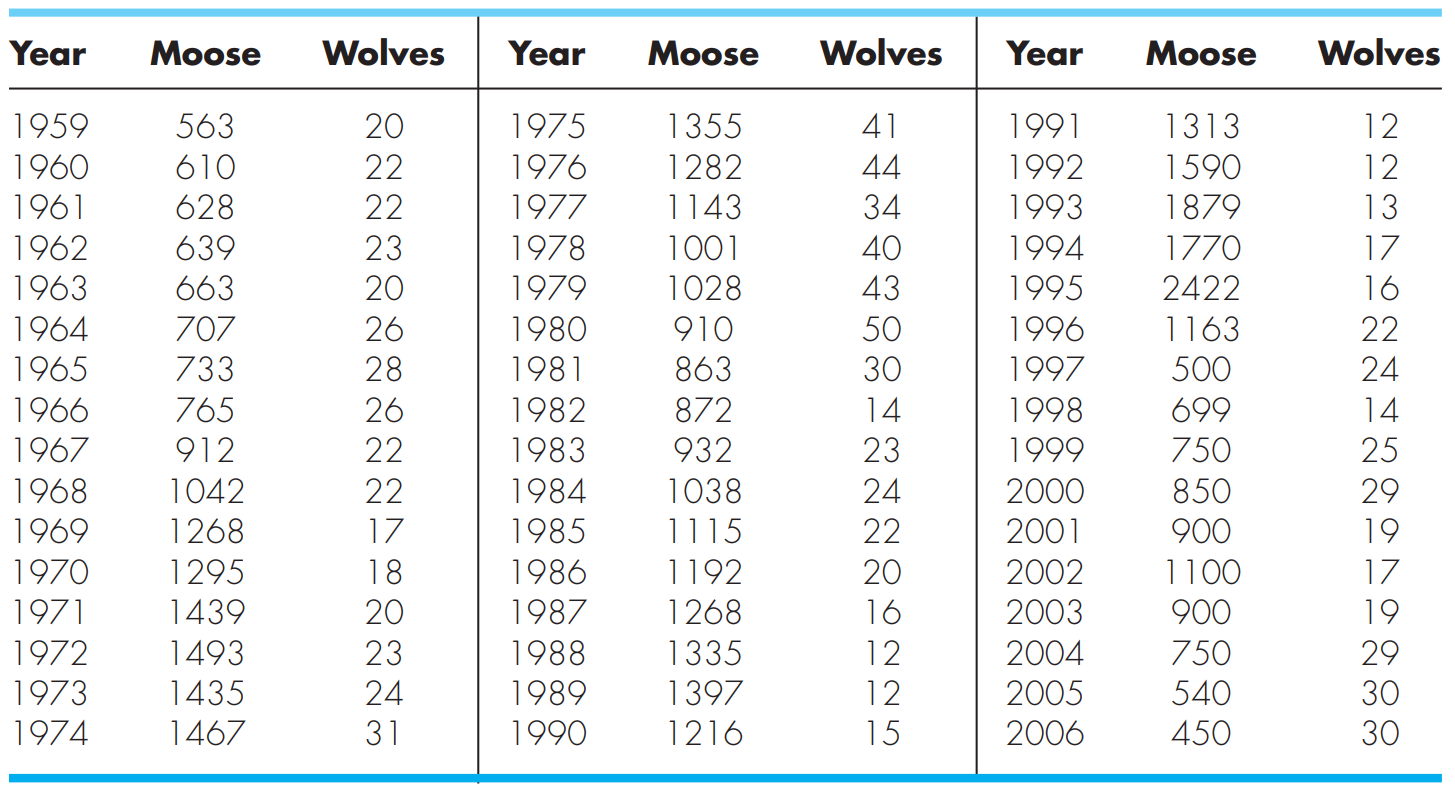
\includegraphics[scale=0.4]{fig_P_22_14}
    \end{figure}

    \begin{multicols}{2}

    \noindent\textbf{22.15} The motion of a damped spring-mass system (Fig. P22.15) is described by the following ordinary differential equation:
    $$
    m \frac{d^{2} x}{d t^{2}}+c \frac{d x}{d t}+k x=0
    $$
    where $x=$ displacement from equilibrium position $(\mathrm{m}),\ t=$ time (s), $m=20-\mathrm{kg}$ mass, and $c=$ the damping coefficient $(\mathrm{N} \cdot \mathrm{s} / \mathrm{m})$. The damping coefficient $c$ takes on three values of 5 (underdamped), 40 (critically damped), and 200 (overdamped). The spring constant $k=20 \mathrm{~N} / \mathrm{m}$.
    The initial velocity is zero, and the initial displacement $x=1 \mathrm{~m}$. Solve this equation using a numerical method over the time period $0 \leq t \leq 15 \mathrm{~s}$. Plot the displacement versus time for each of the three values of the damping coefficient on the same plot.
    
    \begin{figure}[H]
        \centering
        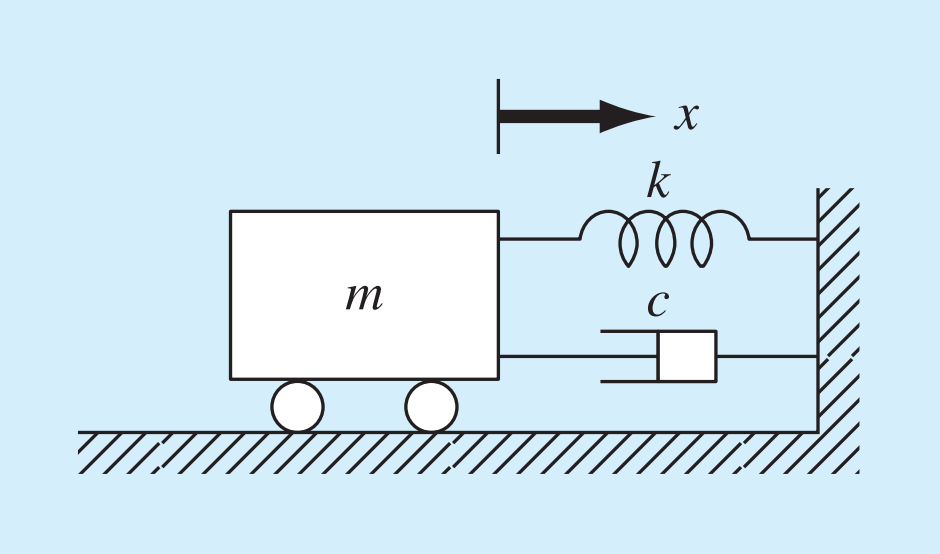
\includegraphics[scale=0.32]{fig_P_22_15}
        \caption{\textsf{}}
        \label{fig:fig_P_22_15}
    \end{figure}\vspace{2mm}

    \noindent\textbf{22.16} A spherical tank has a circular orifice in its bottom through which the liquid flows out (Fig. P22.16). The flow rate through the hole can be estimated as
    $$
    Q_{\text {out }}=C A \sqrt{2 g h}
    $$
    where $Q_{\text {out }}=$ outflow $\left(\mathrm{m}^{3} / \mathrm{s}\right), C=$ an empirically derived coefficient, $A=$ the area of the orifice $\left(\mathrm{m}^{2}\right),\ g=$ the gravitational constant $\left(=9.81 \mathrm{~m} / \mathrm{s}^{2}\right)$, and $h=$ the depth of liquid in the tank.
    Use one of the numerical methods described in this chapter to determine how long it will take for the water to flow out of a $3-\mathrm{m}$ diameter tank with an initial height of $2.75 \mathrm{~m}$. Note that the orifice has a diameter of $3 \mathrm{~cm}$ and $C=0.55$.
    
    \begin{figure}[H]
        \centering
        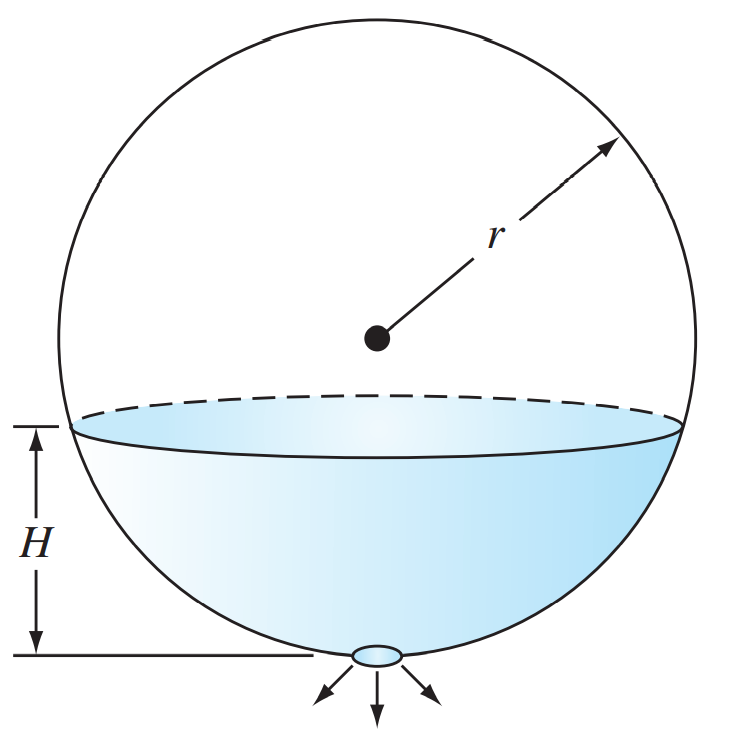
\includegraphics[scale=0.35]{fig_P_22_16}
       \caption{\textsf{A spherical tank.}}\label{fig:fig_P_22_16}
    \end{figure}\vspace{2mm}

    \noindent\textbf{22.17} In the investigation of a homicide or accidental death, it is often important to estimate the time of death. From the experimental observations, it is known that the surface temperature of an object changes at a rate proportional to the difference between the temperature of the object and that of the surrounding environment or ambient temperature.
    This is known as Newton's law of cooling. Thus, if $T(t)$ is the temperature of the object at time $t$, and $T_{a}$ is the constant ambient temperature:
    $$
    \frac{d T}{d t}=-K\left(T-T_{a}\right)
    $$
    where $K>0$ is a constant of proportionality. Suppose that at time $t=0$ a corpse is discovered and its temperature is measured to be $T_{o}$. We assume that at the time of death, the body temperature $T_{d}$ was at the normal value of $37{ }^{\circ} \mathrm{C}$. Suppose that the temperature of the corpse when it was discovered was $29.5{ }^{\circ} \mathrm{C}$, and that two hours later, it is $23.5{ }^{\circ} \mathrm{C}$.
    The ambient temperature is $20{ }^{\circ} \mathrm{C}$.\\
    \textbf{(a)} Determine K and the time of death.\\
    \textbf{(b)} Solve the ODE numerically and plot the results.\vspace{2mm}

    \noindent\textbf{22.18} The reaction $A \rightarrow B$ takes place in two reactors in series. The reactors are well mixed but are not at steady state. The unsteady-state mass balance for each stirred tank reactor is shown below:
    $$
    \begin{aligned}
    \frac{d C A_{1}}{d t} &=\frac{1}{\tau}\left(C A_{0}-C A_{1}\right)-k C A_{1} \\
    \frac{d C B_{1}}{d t} &=\frac{1}{\tau} C B_{1}+k C A_{1} \\
    \frac{d C A_{2}}{d t} &=\frac{1}{\tau}\left(C A_{1}-C A_{2}\right)-k C A_{2} \\
    \frac{d C B_{2}}{d t} &=\frac{1}{\tau}\left(C B_{1}-C B_{2}\right)-k C B_{2}
    \end{aligned}
    $$
    where $C A_{0}=$ concentration of $A$ at the inlet of the first reactor, $C A_{1}=$ concentration of $A$ at the outlet of the first reactor (and inlet of the second), $C A_{2}=$ concentration of $A$ at the outlet of the second reactor,
     $C B_{1}=$ concentration of $B$ at the outlet of the first reactor (and inlet of the second), $C B_{2}=$ concentration of $B$ in the second reactor, $\tau=$ residence time for each reactor, and $k=$ the rate constant for reaction of $A$ to produce $B$.
    If $C A_{0}$ is equal to 20, find the concentrations of $A$ and $B$ in both reactors during their first 10 minutes of operation. Use $k=0.12 / \mathrm{min}$ and $\tau=5 \mathrm{~min}$ and assume that the initial conditions of all the dependent variables are zero.\vspace{2mm}

    \noindent\textbf{22.19} A nonisothermal batch reactor can be described by the following equations:
    $$
    \begin{aligned}
    &\frac{d C}{d t}=-e^{(-10 /(T+273))} C \\
    &\frac{d T}{d t}=1000 e^{(-10 /(T+273))} C-10(T-20)
    \end{aligned}
    $$
    where $C$ is the concentration of the reactant and $T$ is the temperature of the reactor. Initially, the reactor is at $16^{\circ} \mathrm{C}$ and has a concentration of reactant $C$ of $1.0 \mathrm{gmol} / \mathrm{L}$. Find the concentration and temperature of the reactor as a function of time.\vspace{2mm}

    \noindent\textbf{22.20} The following equation can be used to model the deflection of a sailboat mast subject to a wind force:
    $$
    \frac{d^{2} y}{d z^{2}}=\frac{f(z)}{2 E I}(L-z)^{2}
    $$
    where $f(z)=$ wind force, $E=$ modulus of elasticity, $L=$ mast length, and $I=$ moment of inertia. Note that the force varies with height according to
    $$
    f(z)=\frac{200 z}{5+z} e^{-2 z / 30}
    $$
    Calculate the deflection if $y=0$ and $d y / d z=0$ at $z=0$. Use parameter values of $L=30, E=1.3 \times 10^{8}$, and\vspace{2mm}

    \noindent\textbf{22.21} A pond drains through a pipe as shown in Fig. P22.21. Under a number of simplifying assumptions, the following differential equation describes how depth changes with time:$$\frac{d h}{d t}=-\frac{\pi d^{2}}{4 A(h)} \sqrt{2 g(h+e)}$$
    where $h=\operatorname{depth}(\mathrm{m}), t=$ time $(\mathrm{s}), d=$ pipe diameter $(\mathrm{m})$, $A(h)=$ pond surface area as a function of depth $\left(\mathrm{m}^{2}\right), g=$ gravitational constant $\left(=9.81 \mathrm{~m} / \mathrm{s}^{2}\right)$, 
    and $e=$ depth of pipe outlet below the pond bottom $(\mathrm{m})$. Based on the following area-depth table, solve this differential equation to determine how long it takes for the pond to empty, given that $h(0)=6 \mathrm{~m}, d=0.25 \mathrm{~m}, e=1 \mathrm{~m}$.

    \begin{figure}[H]
        \centering
        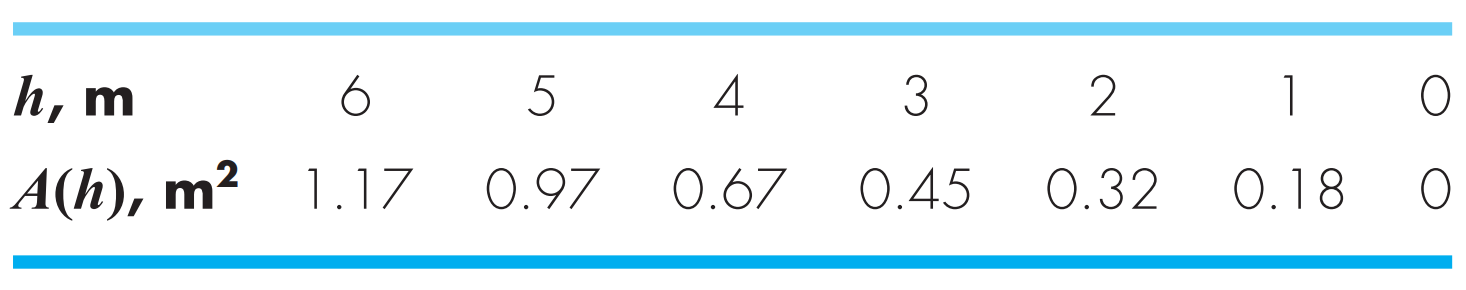
\includegraphics[scale=0.2]{fig_P_22_21_1}
        \label{fig:fig_P_22_21_1}
    \end{figure}
    
    \begin{figure}[H]
        \centering
        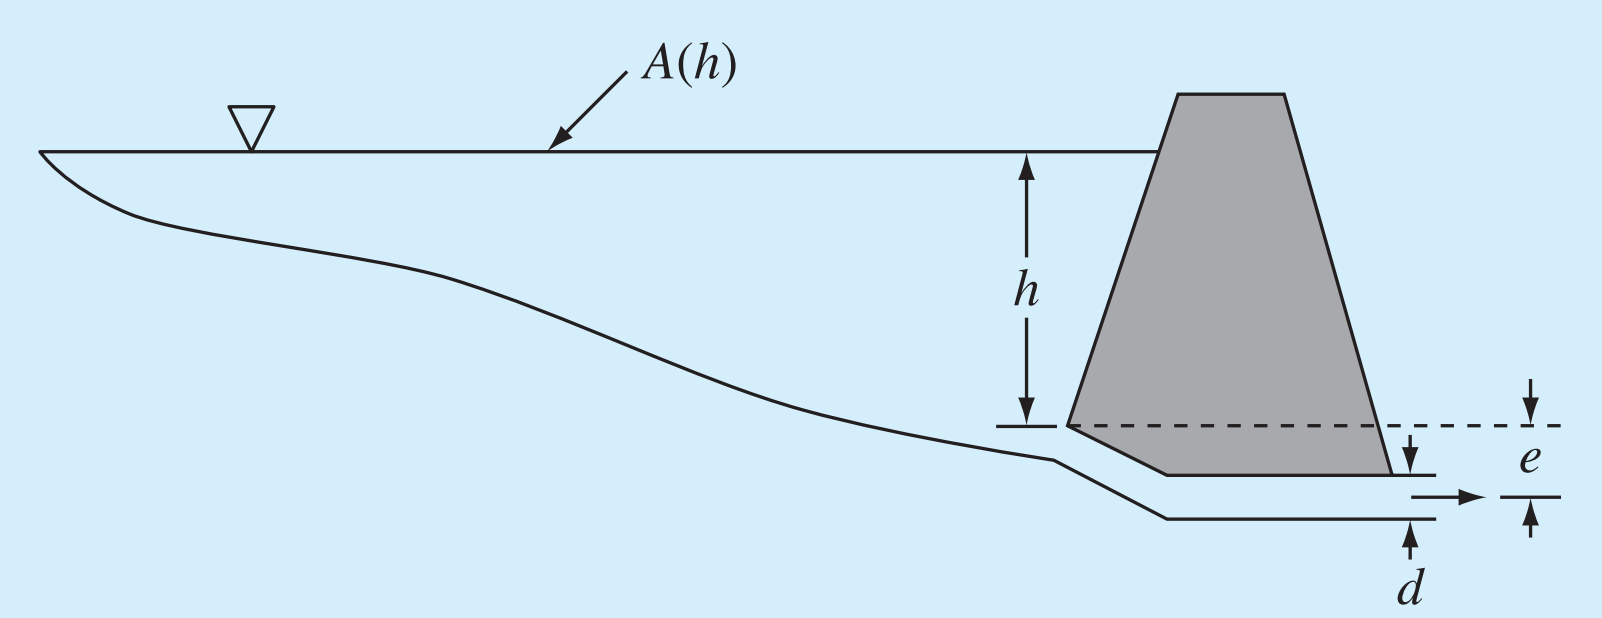
\includegraphics[scale=0.2]{fig_P_22_21}
        \caption{\textsf{}}
        \label{fig:fig_P_22_21}
    \end{figure}\vspace{2mm}

    \noindent\textbf{22.22} Engineers and scientists use mass-spring models to gain insight into the dynamics of structures under the influence of disturbances such as earthquakes. Figure P22.22 shows such a representation for a three-story building. For this case, the analysis is limited to horizontal motion of the structure. Using Newton's second law, force balances can be developed for this system as
    $$
    \begin{aligned}
    &\frac{d^{2} x_{1}}{d t^{2}}=-\frac{k_{1}}{m_{1}} x_{1}+\frac{k_{2}}{m_{1}}\left(x_{2}-x_{1}\right) \\
    &\frac{d^{2} x_{2}}{d t^{2}}=\frac{k_{2}}{m_{2}}\left(x_{1}-x_{2}\right)+\frac{k_{3}}{m_{2}}\left(x_{3}-x_{2}\right) \\
    &\frac{d^{2} x_{3}}{d t^{2}}=\frac{k_{3}}{m_{3}}\left(x_{2}-x_{3}\right)
    \end{aligned}
    $$
    Simulate the dynamics of this structure from $t=0$ to $20 \mathrm{~s}$, given the initial condition that the velocity of the ground floor is $d x_{1} / d t=1 \mathrm{~m} / \mathrm{s}$, and all other initial values of displacements and velocities are zero. Present your results as two time-series plots of \textbf{(a)} displacements and \textbf{(b)} velocities. In addition, develop a     three-dimensional phase-plane plot of the displacements.
    
    \begin{figure}[H]
        \centering
        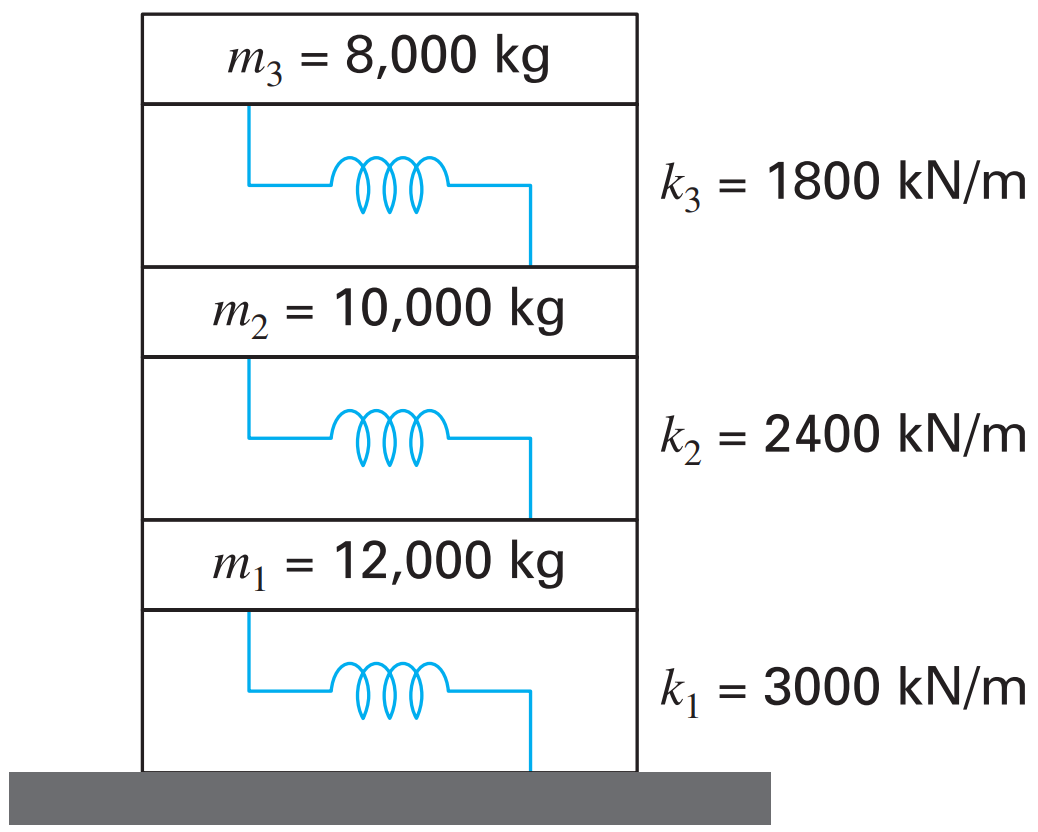
\includegraphics[scale=0.2]{fig_P_22_22}
        \caption{\textsf{}}
        \label{fig:fig_P_22_22}
    \end{figure}\vspace{2mm}

    \noindent\textbf{22.23} Repeat the the same simulations as in Section 22.6
    for the Lorenz equations but generate the solutions with the
    midpoint method.\vspace{2mm}

    \noindent\textbf{22.24} Perform the same simulations as in Section 22.6 for
    the Lorenz equations but use a value of $r = 99.96$. Compare
    your results with those obtained in Section 22.6.\vspace{2mm}
    \end{multicols}




\end{document}